\documentclass[14pt,a4paper,oneside,openany]{extbook}
\let\cleardoublepage\clearpage

\input{preamble.tex}

\newif\ifomitvalidationchapter
\omitvalidationchapterfalse
\ifdefined\omitvalidationchapterdraft
  \omitvalidationchaptertrue
\fi

\begin{document}

% Нумерация страниц начинается с листа «СОДЕРЖАНИЕ» (п. 4.3.1)
% Нумерация сквозная по всему документу, включая приложения.
% Титульный лист, задание и аннотация оформляются в ИСУ ИТМО отдельно.
% Если нужно скорректировать стартовый номер (например, 4 если перед
% содержанием идут 3 страницы из ИСУ) — измените число ниже:
\setcounter{page}{4}  % Титульный лист + задание + аннотация = 3 стр. в ИСУ ИТМО

% СОДЕРЖАНИЕ — отдельный лист, без номера раздела (п. 4.4.1, 3.4)
\chapter*{СОДЕРЖАНИЕ}
\markboth{СОДЕРЖАНИЕ}{}
\vspace{-3.5cm}
{%
  \renewcommand{\contentsname}{}%
  \tableofcontents
}

% Список сокращений и условных обозначений (п. 3.2, 4.8)
\chapter*{СПИСОК СОКРАЩЕНИЙ И УСЛОВНЫХ ОБОЗНАЧЕНИЙ}
\addcontentsline{toc}{chapter}{СПИСОК СОКРАЩЕНИЙ И УСЛОВНЫХ ОБОЗНАЧЕНИЙ}
\setlength{\parindent}{0pt}
% Перечень располагается столбцом, слева без абзацного отступа в алфавитном порядке,
% справа через тире — расшифровка, без знаков препинания в конце строки (п. 4.8.4)
\setlength{\LTpre}{0pt}
\setlength{\LTpost}{0pt}
\begin{longtable}{@{}p{2.8cm}@{\hspace{0.5em}---\hspace{0.5em}}p{12.4cm}@{}}
ADDIE & Analyze, Design, Develop, Implement, Evaluate (методология проектирования курсов)\\[0.5em]
API & Application Programming Interface (интерфейс программирования приложений)\\[0.5em]
B2B & Business-to-Business (бизнес-модель)\\[0.5em]
BD & Backward Design (методология «обратного проектирования» курса)\\[0.5em]
BFF & Backend-for-Frontend (паттерн архитектуры)\\[0.5em]
CAC & Customer Acquisition Cost (стоимость привлечения клиента)\\[0.5em]
CI/CD & Continuous Integration / Continuous Delivery (непрерывная интеграция и доставка)\\[0.5em]
CVM & Customer Value Management (управление ценностью клиента)\\[0.5em]
DAG & Directed Acyclic Graph (ориентированный ациклический граф)\\[0.5em]
GPU & Graphics Processing Unit (графический процессор)\\[0.5em]
IRR & Internal Rate of Return (внутренняя норма доходности)\\[0.5em]
JTBD & Jobs To Be Done (методология исследования потребностей)\\[0.5em]
KPI & Key Performance Indicator (ключевой показатель эффективности)\\[0.5em]
LLM & Large Language Model (большая языковая модель)\\[0.5em]
LMS & Learning Management System (система управления обучением)\\[0.5em]
LOI & Letter of Intent (письмо о намерениях)\\[0.5em]
LTV & Lifetime Value (пожизненная ценность клиента)\\[0.5em]
MVP & Minimum Viable Product (минимально жизнеспособный продукт)\\[0.5em]
NPS & Net Promoter Score (индекс потребительской лояльности)\\[0.5em]
NPV & Net Present Value (чистая приведённая стоимость)\\[0.5em]
RAG & Retrieval-Augmented Generation (генерация с~дополнением поиском)\\[0.5em]
REST & Representational State Transfer (архитектурный стиль API)\\[0.5em]
ROI & Return on Investment (рентабельность инвестиций)\\[0.5em]
SAM & Successive Approximation Model (итеративная методология проектирования курсов)\\[0.5em]
SAM & Serviceable Addressable Market (доступный рынок) [в~контексте рыночного анализа]\\[0.5em]
SOM & Serviceable Obtainable Market (реально достижимый рынок)\\[0.5em]
SUS & System Usability Scale (шкала удобства использования системы)\\[0.5em]
TAM & Total Addressable Market (общий доступный рынок)\\[0.5em]
TTS & Text-to-Speech (синтез речи)\\[0.5em]
ВКР & выпускная квалификационная работа\\[0.5em]
ИИ & искусственный интеллект\\[0.5em]
ИС & интеллектуальная собственность\\[0.5em]
ЛМС & система управления обучением (эквивалент LMS)\\[0.5em]
ЛПР & лицо, принимающее решения
\end{longtable}
\setlength{\parindent}{1.25cm}

\cleardoublepage

% Список терминов и определений (п. 3.2, 4.9)
\chapter*{ТЕРМИНЫ И ОПРЕДЕЛЕНИЯ}
\addcontentsline{toc}{chapter}{ТЕРМИНЫ И ОПРЕДЕЛЕНИЯ}
\setlength{\parindent}{0pt}
% Перечень располагается столбцом, слева без абзацного отступа в алфавитном порядке,
% справа через тире — определение, без знаков препинания в конце строки (п. 4.9.2)
% Термины пишутся без жирного шрифта
\setlength{\LTpre}{0pt}
\setlength{\LTpost}{0pt}
\begin{longtable}{@{}P{4.8cm}@{\hspace{0.5em}—\hspace{0.5em}}P{10.4cm}@{}}
Source provenance & фиксация происхождения результата с указанием исходного документа, фрагмента источника, шага агентного конвейера и блока сгенерированного курса\\[0.5em]
Агентный конвейер & управляемая последовательность узлов ИИ-методиста, где каждый узел выполняет отдельный этап от анализа источника до финальной верификации\\[0.5em]
Знак качества & пороговый статус финальной верификации, рассчитанный по доле подтверждённых утверждений в таблице свидетельств\\[0.5em]
Таблица свидетельств & машиночитаемая таблица проверки фактических утверждений, содержащая утверждение, источник, статус подтверждения и комментарий проверки
\end{longtable}
\setlength{\parindent}{1.25cm}

\cleardoublepage

% Основной текст работы (п. 3.2)
\mainmatter
\chapter*{ВВЕДЕНИЕ}
\addcontentsline{toc}{chapter}{ВВЕДЕНИЕ}
\sloppy

Большие языковые модели (LLM) всё активнее применяются для~автоматизации
рутинных операций при~проектировании образовательных материалов.
Мировой рынок корпоративного обучения, по~оценкам аналитических агентств,
превысит \$51~млрд к~2030~году~\cite{edtech_market_report_2024}.
Главный сдерживающий фактор роста~--- высокая стоимость
и~длительность создания качественного учебного контента.
Средний цикл разработки одного корпоративного курса силами методиста-эксперта
составляет от~нескольких дней до~нескольких недель и~требует педагогических
компетенций, которыми не~всегда обладают эксперты предметной области.

Существующие ИИ-инструменты для~ускоренной подготовки курсов (Coursebox~AI, iSpring~AI)
предоставляют одношаговую генерацию на~основе единственного промпта и,
как~правило, не~поддерживают научно обоснованные методологии проектирования учебного процесса
(ADDIE, SAM, Backward~Design).
Мультиагентные LLM-конвейеры для~решения этой задачи
остаются малоизученными: отсутствуют систематические сравнения архитектур
на~воспроизводимом российском корпусе документов и~внешнем зарубежном сравнительном контуре, а~также воспроизводимые бенчмарки
с~привязкой не~только к~таксономии Блума, но и~к~согласованности курса,
качеству онлайн-курса и~переносу обучения в~практику.

\textbf{Объект исследования}~--- образовательная платформа Adapstory~(AI~LMS),
предоставляющая инструменты создания и~управления учебными курсами
для~B2B-клиентов.

\textbf{Предмет исследования}~--- микросервис ИИ-методист:
интеллектуальный проактивный методический ассистент, поддерживающий
методиста, эксперта и~разработчика курса при~создании, упаковке и~актуализации
образовательных продуктов на~основе LLM с~применением мультиагентной
оркестрации.

\textbf{Цель работы}~--- разработка и~валидация интеллектуального
методического ассистента, сокращающего рутинную нагрузку при~подготовке
структуры и~черновых материалов учебных курсов на~основе входных
документов заказчика при~сохранении за~человеком методического решения
и~контроля качества, измеримого по~таксономии Блума.

Для~достижения цели поставлены следующие задачи:
\begin{enumerate}
  \item провести анализ предметной области: Customer~Development с~B2B-аудиторией,
    продуктовый обзор конкурентов и~систематический обзор научных подходов;
  \item оценить рыночный потенциал решения (TAM/SAM/SOM) и~сформулировать
    исследовательские гипотезы;
  \item спроектировать мультиагентную архитектуру конвейера поддержки
    проектирования курсов
    и~обосновать выбор технологического стека через воспроизводимые эксперименты;
  \item реализовать систему: контур обработки документов (Document~Ingestion~Pipeline, Haystack~2.x),
    граф агентов LangGraph, LLM~Gateway, FastAPI-микросервис;
  \item провести валидацию системы: автоматизированную оценку
    (Ragas, покрытие уровней таксономии Блума),
    экспертный слепой тест (n~=~5--8~методистов) и~пилотное исследование с~B2B-клиентами;
  \item оценить бизнес-потенциал: unit-экономику, финансовую модель
    и~провести Customer~Development для~подтверждения соответствия решения выявленной проблеме.
\end{enumerate}

\textbf{Научная новизна} работы состоит в~следующем:
предложена и~экспериментально верифицирована мультиагентная архитектура
поддержки проектирования учебных курсов, впервые сочетающая
(1)~вариативную методологическую модель проектирования (ADDIE / SAM / Backward~Design)
как~переключаемый системный промпт,
(2)~графовую оркестрацию с~сохраняемым состоянием и~участием человека
(LangGraph~StateGraph),
и~(3)~RAG-слой на~воспроизводимом российском корпусе открытых
и~официальных документов с~отдельным зарубежным сравнительным контуром
(Qdrant~+~deepvk/USER-bge-m3).
Архитектура превосходит одношаговую базовую конфигурацию
по~достоверности относительно источника и~покрытию уровней
таксономии Блума.

\textbf{Положения, выносимые на защиту:}
\begin{enumerate}
  \item Мультиагентный конвейер с~вариативной методологической моделью
    (ADDIE/SAM/Backward~Design) сокращает время подготовки первого
    методического черновика курса с~X~часов до~Y~минут
    при~сохранении покрытия уровней таксономии Блума $\geq 70\%$.
  \item Графовая архитектура с~сохраняемым состоянием (LangGraph)
    обеспечивает статистически значимо более высокое качество структуры курса
    по~сравнению с~одношаговым подходом на~той же базовой LLM.
  \item Система прошла этап подтверждения соответствия решения проблеме:
    $N$~B2B-пилотов
    подтверждены письмами о~готовности от~ЛПР.
\end{enumerate}

Текущее состояние проекта: разработан и~протестирован MVP,
включающий контур обработки документов и~агентный конвейер
поддержки проектирования курса с~методологией~ADDIE; проведены
B2B-интервью и~получены LOI-письма от~корпоративных заказчиков.

Работа состоит из~введения,
\ifomitvalidationchapter
трёх глав, заключения,
\else
четырёх глав, заключения,
\fi
раздела об~использовании ИИ, списка использованных источников
и~десяти приложений.
Глава~1 содержит анализ предметной области и~постановку задачи.
Глава~2 описывает дизайн эксперимента и~обоснование выбора технологий.
Глава~3 посвящена технической реализации системы.
\ifomitvalidationchapter
\else
Глава~4 содержит результаты валидации, анализ ограничений
и~бизнес-оценку.
\fi

\chapter{АНАЛИЗ ПРЕДМЕТНОЙ ОБЛАСТИ И ПОСТАНОВКА ЗАДАЧИ}

% ─────────────────────────────────────────────────────────────────
\section{Проблема и её масштаб}
% ─────────────────────────────────────────────────────────────────

\subsection{Болевые точки авторов курсов}

Разработка корпоративного учебного курса остаётся трудоёмким и слабо
масштабируемым процессом. Даже при наличии готового экспертного материала
необходимо определить целевую аудиторию, сформулировать учебные цели,
разбить содержание на модули и уроки, подобрать формат подачи,
подготовить оценочные материалы и синхронизировать всё это
с~требованиями LMS.
По~оценке Chapman Alliance, производство одного часа eLearning-контента
требует от~42 до~490 часов работы в~зависимости от~сложности сценария,
мультимедийности и глубины методической проработки; для большинства
практических проектов реалистичный коридор составляет 40--200 часов
на~один час готового обучения~\cite{chapman_elearning_hours_2010}.

Для российского B2B-сегмента проблема усугубляется дополнительно.

\begin{itemize}
  \item \textbf{Дефицит методических компетенций.} Эксперт предметной
    области знает материал, но не всегда умеет переводить знание
    в~педагогически корректную структуру курса. Другой проблемой становится нехватка или перегрузка специалистов
    в~области методики преподавания. У компаний зачастую нет финансовой возможности иметь собственный методический отдел.
  \item \textbf{Высокая стоимость внешней разработки.} На рынке
    корпоративного обучения разработка одного курса силами подрядчика
    обычно оценивается в диапазоне 100--300~тыс.\ руб.\ за проект,
    что делает частое обновление контента экономически невыгодным
    для малого и среднего бизнеса~\cite{smart_ranking_elearning_2024}.
  \item \textbf{Быстрое устаревание источников.} Регламенты, продуктовые
    описания и внутренние правила обновляются быстрее, чем команда
    успевает вручную пересобирать учебные материалы, из-за чего курс
    быстро расходится с~актуальной версией исходного документа.
\end{itemize}

\subsection{Разрыв между экспертизой и образовательной упаковкой}

В корпоративной среде инициатором
курса обычно выступает владелец продукта, руководитель функции, HR или
L\&D-менеджер. Первый хорошо знает предметную область, второй понимает
бизнес-контекст, однако ни один из них не обязательно владеет
инструментами педагогического дизайна на уровне, достаточном для создания
масштабируемого цифрового курса.

На практике это проявляется так: черновой
материал остаётся на уровне «экспертного конспекта» без явных
учебных результатов и уровней освоения. Структура курса
строится от имеющихся документов, а не от целей обучения, что снижает
практическую ценность. Сопровождение же требует
подключения методиста, зачастую не входящего в команду.

\subsection{Подтверждение проблемы: результаты исследования клиентов}

Для первичной проверки гипотез о проблеме проведено 20 глубинных
B2B-интервью с~HR-специалистами, L\&D-менеджерами, методистами и
корпоративными тренерами по~подходу Mom~Test~\cite{fitzpatrick_mom_test_2013}.
Руководство интервью, логика кодирования ответов и шаблон таблицы выводов
вынесены в приложение~А.

Количественные результаты:

\begin{itemize}
  \item \textbf{70\,\%} респондентов называют время подготовки курса
    главным ограничением запуска нового обучения;
  \item \textbf{50\,\%} респондентов уже привлекают внешних подрядчиков
    или отдельных методистов для упаковки материала;
  \item \textbf{60\,\%} готовы рассмотреть ИИ-инструмент как часть
    текущего процесса разработки, если он не ухудшает качество
    структуры и позволяет сохранить контроль над итоговым результатом.
\end{itemize}

Распределение ответов респондентов представлено на рисунке~\ref{fig:custdev-bars}.

\begin{figure}[htbp]
\centering
\begin{tikzpicture}
\begin{axis}[
    xbar,
    width=0.85\textwidth,
    height=5cm,
    xlabel={Доля респондентов, \%},
    xmin=0, xmax=100,
    ytick=data,
    yticklabels={
        {Готовы рассмотреть ИИ-инструмент},
        {Привлекают внешних подрядчиков},
        {Время разработки --- главное ограничение}
    },
    y tick label style={font=\small, anchor=east},
    nodes near coords,
    nodes near coords align={horizontal},
    nodes near coords style={font=\small, append after command={node[anchor=west]{\,\%}}},
    bar width=14pt,
    enlarge y limits=0.35,
    every axis plot/.append style={fill=teal!80!black, draw=teal!60!black},
]
\addplot coordinates {(60,0) (50,1) (70,2)};
\end{axis}
\end{tikzpicture}
\caption{Результаты Customer Development (n=20 B2B-интервью)}
\label{fig:custdev-bars}
\end{figure}


Качественный вывод: обучающиеся находятся в
профиците информации и дефиците времени. Отсюда запрос --- быстро превратить регламент,
брендбук или продуктовый бриф в обучение с понятной логикой, проверяемыми
учебными целями и практическим результатом.

\subsection[Решенческие интервью и критерии решения]{Решенческие интервью и критерии соответствия решения проблеме}

Серия решенческих интервью проведена на базе функционального прототипа ИИ-методиста
(сценарий демонстрации --- приложение~Б). Проверяемые
критерии соответствия решения проблеме:

\begin{enumerate}
  \item готов ли руководитель L\&D-отдела встроить систему
    в~текущую ручную стадию подготовки черновой структуры курса
    как~инструмент ускорения и~снятия рутины;
  \item готов ли методист использовать систему на реальном документе
    своей организации;
  \item экономически эффективно ли решение по отношению к
    стоимости аутсорс-разработки или внутреннего
    методического ресурса.
\end{enumerate}

\subsection{Рыночный контекст: TAM / SAM / SOM}

Глобальный рынок онлайн-обучения растёт:
по оценке Grand View Research, его объём составил
\$299{.}67~млрд в~2024~году и может достичь \$842{.}64~млрд к~2030~году
при CAGR около 19\,\%~\cite{grandview_elearning_2025}. Это задаёт
широкий TAM для решений, ускоряющих подготовку цифровых
образовательных материалов.

Для оценки сегмента в~России в работе используется
более консервативная логика. По данным Smart Ranking, объём
российского EdTech-рынка в~2023~году достиг 119{.}33~млрд~руб.,
а доля сегмента «разработчики и платформы» составляла 13\,\%
от общей структуры рынка~\cite{smart_ranking_elearning_2024}.
Актуальные обзоры СберОбразования за 2025~год также фиксируют
рост внимания к ИИ-инструментам, персонализации и автоматизации
образовательных процессов~\cite{sber_education_trends_q2_2025,sber_education_trends_q3_2025}.
Этот слой ближе всего по природе
к ИИ-методисту; рынок инструментов поддержки
разработки курсов оценивается примерно в~15{.}5~млрд~руб.

При целевой доле 0{.}1\,\% от~SAM в~горизонте трёх лет
SOM составляет около 15{.}5~млн~руб.\ в год. При базовой B2B-подписке порядка
15~тыс.\ руб.\ в месяц это соответствует примерно
85--90 активным корпоративным клиентам. Такой масштаб достижим
для нишевого B2B-продукта.

Структура рыночной оценки показана на рисунке~\ref{fig:tam-sam-som}.

\begin{figure}[htbp]
\centering
\begin{tikzpicture}
% TAM — widest
\fill[teal!70!black, rounded corners=2pt] (-6,0) rectangle (6,1.2);
\node[font=\bfseries\small, text=white] at (0,0.6) {TAM (глобальный): \$842{,}64 млрд к~2030 г.};

% SAM — medium
\fill[teal!50!black, rounded corners=2pt] (-4,-1.8) rectangle (4,-0.6);
\node[font=\bfseries\small, text=white] at (0,-1.2) {SAM (EdTech-инструменты, РФ): 15{,}5 млрд руб.};

% SOM — narrowest
\fill[teal!30!black, rounded corners=2pt] (-2.2,-3.6) rectangle (2.2,-2.4);
\node[font=\bfseries\small, text=white] at (0,-3.0) {SOM (3 года): 15{,}5 млн руб.};

% Connecting dashed lines (funnel edges)
\draw[gray, dashed, thick] (-6,0) -- (-4,-0.6);
\draw[gray, dashed, thick] (6,0) -- (4,-0.6);
\draw[gray, dashed, thick] (-4,-1.8) -- (-2.2,-2.4);
\draw[gray, dashed, thick] (4,-1.8) -- (2.2,-2.4);
\end{tikzpicture}
\caption{Оценка рынка: TAM / SAM / SOM}
\label{fig:tam-sam-som}
\end{figure}


% ─────────────────────────────────────────────────────────────────
\section{Анализ существующих продуктов}
% ─────────────────────────────────────────────────────────────────

\subsection{Прямые конкуренты}

\textbf{Coursebox~AI} позиционируется как конструктор курсов на~основе ИИ и
позволяет преобразовывать документы, слайды, видео и URL в курс,
автоматически генерировать тесты, видео, изображения и публиковать
результат в собственную LMS либо экспортировать в SCORM/LTI
форматах~\cite{coursebox_ai_2024}. Это один из наиболее близких
по~ценностному предложению продукт на~рынке.
Однако его логика остаётся в~первую очередь ориентированной
на~быструю упаковку содержимого:
сильная сторона продукта --- скорость, а не явная
педагогическая методология или контроль корректности фактов
по отношению к исходному документу.

\textbf{Articulate 360 AI} добавляет ИИ-функции в зрелую среду
корпоративного контента: создание структуры курса, чернового текста,
перевода, изображений и озвучки внутри экосистемы Articulate.
Продукт хорошо встроен в привычный рабочий процесс методиста,
но остаётся инструментом повышения производительности разработчика курса,
а не самостоятельным методическим конвейером с RAG-слоем,
проверкой фактов и локальным развёртыванием~\cite{articulate_ai_2025}.

\textbf{iSpring Suite AI} развивает похожую траекторию:
в~2025~году в продукт добавлены AI Course Creation Helper,
AI Translator, AI Image Generator, а также функции синтеза речи и
другие инструменты ускорения разработки курса~\cite{ispring_suite_ai_2026}.
Сильной стороной iSpring является зрелая экосистема для корпоративного
обучения и русскоязычный рынок. Ограничение состоит в том, что ИИ
остаётся надстройкой над средой разработки контента, а не автономным
мультиагентным конвейером, принимающим на вход первичный документ
и проводящим его через полную цепочку анализа, проектирования и
обновления курса.

\textbf{Synthesia} лидирует в классе ИИ-видеогенерации для обучения
и корпоративных коммуникаций: её ценность сосредоточена в создании
аватарных роликов, озвучки и мультиязычного видео-контента
для обучения и L\&D-задач~\cite{synthesia_ai_training_2025}.
Но Synthesia не закрывает задачу проектирования учебной структуры.

\subsection{Смежные решения}

\textbf{Google NotebookLM} --- сильный смежный продукт для работы
с источниками, который умеет строить краткие выжимки, аудиообзоры
и видеообзоры по загруженным материалам. В~2025~году Google
расширил генерацию аудио и видео обзоров до 80+ языков, сделав
их заметно реалистичнее и полезнее для изучения сложных источников
~\cite{notebooklm_audio_2025}. Однако NotebookLM не предназначен
для создания LMS-совместимой структуры курса, педагогического
дизайна и контроля соответствия учебных целей.

\textbf{GetCourse} является одним из крупнейших российских игроков
рынка LMS/онлайн-школ: платформа сообщает о 50{,}000+ клиентах,
16~млн учеников и совокупном обороте школ на платформе в
158~млрд~руб.\ за 2025~год~\cite{getcourse_platform_2026}.
Для настоящей работы GetCourse важен как ориентир класса систем, в которые ИИ-методист потенциально
может встраиваться как сервис генерации и обновления курса.

\subsection{Сравнительная матрица}

В таблице~\ref{tab:competitors} приведено сравнение решений по критериям,
которые оказались значимыми в исследовании клиентов: способность работать
от исходного документа, наличие встроенной педагогической логики,
поддержка русскоязычного контента, суверенитет данных, автоматическое
обновление содержания и интеграция с LMS-средой.

\begin{table}[h!]
  \caption{Сравнительный анализ конкурентных решений}
  \label{tab:competitors}
  \centering
  \small
  \begin{tabular}{|p{3.2cm}|c|c|c|c|c|}
  \hline
  \textbf{Критерий}
    & \textbf{Coursebox}
    & \textbf{Articulate~AI}
    & \textbf{iSpring~AI}
    & \textbf{Synthesia}
    & \textbf{ИИ-методист} \\
  \hline
  Генерация курса из документа
    & +
    & $\pm$
    & $\pm$
    & ---
    & \textbf{+} \\
  \hline
  Явная методология (ADDIE / SAM / BD)
    & ---
    & ---
    & ---
    & ---
    & \textbf{+} \\
  \hline
  Русскоязычный контент
    & $\pm$
    & $\pm$
    & +
    & $\pm$
    & \textbf{+} \\
  \hline
  Локальное развёртывание и~суверенитет данных
    & ---
    & ---
    & ---
    & ---
    & \textbf{+} \\
  \hline
  ИИ-аудио / видео
    & +
    & +
    & +
    & \textbf{+}
    & + \\
  \hline
  Проверка фактов по источнику
    & ---
    & ---
    & ---
    & ---
    & \textbf{+} \\
  \hline
  Автоматическое обновление курса
    & $\pm$
    & ---
    & ---
    & ---
    & \textbf{+} \\
  \hline
  Ревью с~участием человека
    & +
    & +
    & +
    & +
    & \textbf{+} \\
  \hline
  Интеграция с LMS-потоком разработки
    & +
    & +
    & +
    & ---
    & \textbf{+} \\
  \hline
  \end{tabular}
\end{table}

Визуализация сравнения в форме радарной диаграммы приведена на рисунке~\ref{fig:competitor-radar}.

\begin{figure}[htbp]
\centering
\begin{tikzpicture}
\begin{polaraxis}[
    name=radar,
    width=0.78\textwidth,
    height=0.78\textwidth,
    xtick={0,60,120,180,240,300},
    xticklabels={
        {Генерация\\из документа},
        Методология,
        {Русский\\язык},
        {Локальное\\развёртывание},
        {Проверка\\фактов},
        {Автоматическое\\обновление}
    },
    xticklabel style={font=\footnotesize, anchor=center, align=center, inner sep=8pt},
    ymin=0, ymax=1.2,
    ytick={0.25,0.5,0.75,1},
    yticklabels={},
    y grid style={gray!30},
    x grid style={gray!50, thick},
    grid=both,
    legend style={
        at={(0.5,-0.1)},
        anchor=north,
        font=\footnotesize,
        cells={anchor=west},
        legend columns=3,
        column sep=6pt,
    },
]

% ИИ-методист (рисуем первым — фон)
\addplot[teal!70!black, very thick, mark=*, mark size=2.5pt, fill=teal!12!white]
    coordinates {(0,1)(60,1)(120,1)(180,1)(240,1)(300,1)(360,1)};
\addlegendentry{ИИ-методист}

% Coursebox
\addplot[blue!70!black, thick, mark=square*, mark size=2.5pt]
    coordinates {(0,1)(60,0)(120,0.5)(180,0)(240,0)(300,0.5)(360,1)};
\addlegendentry{Coursebox}

% Articulate AI
\addplot[red!70!black, thick, mark=triangle*, mark size=2.5pt]
    coordinates {(0,0.5)(60,0)(120,0.5)(180,0)(240,0)(300,0)(360,0.5)};
\addlegendentry{Articulate AI}

% iSpring AI
\addplot[orange!80!black, thick, mark=diamond*, mark size=2.5pt]
    coordinates {(0,0.5)(60,0)(120,1)(180,0)(240,0)(300,0)(360,0.5)};
\addlegendentry{iSpring AI}

% Synthesia
\addplot[purple!70!black, thick, mark=pentagon*, mark size=2.5pt]
    coordinates {(0,0)(60,0)(120,0.5)(180,0)(240,0)(300,0)(360,0)};
\addlegendentry{Synthesia}

% Подписи шкалы вдоль одного луча (90° = вверх-вправо, ось "Методология")
\node[font=\tiny, fill=white, inner sep=1pt, text=gray!70!black] at (axis cs:30,0.25) {0{,}25};
\node[font=\tiny, fill=white, inner sep=1pt, text=gray!70!black] at (axis cs:30,0.5) {0{,}5};
\node[font=\tiny, fill=white, inner sep=1pt, text=gray!70!black] at (axis cs:30,0.75) {0{,}75};
\node[font=\tiny, fill=white, inner sep=1pt, text=gray!70!black] at (axis cs:30,1.0) {1{,}0};

\end{polaraxis}
\end{tikzpicture}
\caption{Радарная диаграмма сравнения решений}
\label{fig:competitor-radar}
\end{figure}


\subsection{Пробел между проблемой и существующими решениями}

Рынок предлагает и стартапы, и зрелые продукты
для ускорения создания обучения. Однако сохраняется разрыв между генерацией учебных материалов и адаптацией к контексту каждого обучающегося.

Ни одно из рассмотренных решений не закрывает одновременно четыре
требования корпоративного B2B-заказчика:

\begin{enumerate}
  \item работу от внутреннего документа организации как от первичного
    источника;
  \item поддерживать методическую логику проектирования курса для достижения целей обучения;
  \item возможность локального развёртывания и контроля данных;
  \item механизм повторной генерации и обновления курса при изменении
    исходного источника.
\end{enumerate}

Позиционирование решений на карте приведено на рисунке~\ref{fig:positioning-map}.

\begin{figure}[htbp]
\centering
\begin{tikzpicture}
\begin{axis}[
    width=0.85\textwidth,
    height=0.7\textwidth,
    xlabel={Методическая глубина},
    ylabel={Суверенитет данных},
    xmin=0, xmax=10,
    ymin=0, ymax=10,
    grid=major,
    grid style={gray!30},
    xlabel style={font=\small},
    ylabel style={font=\small},
    tick label style={font=\small},
    clip=false,
]

% Regular competitors
\addplot[only marks, mark=*, mark size=3pt, teal!60!black]
    coordinates {(3,1)};
\node[anchor=south west, font=\scriptsize] at (axis cs:3.2,1.1) {Coursebox AI};

\addplot[only marks, mark=*, mark size=3pt, teal!60!black]
    coordinates {(4,1)};
\node[anchor=south west, font=\scriptsize] at (axis cs:4.2,1.1) {Articulate AI};

\addplot[only marks, mark=*, mark size=3pt, teal!60!black]
    coordinates {(4,2)};
\node[anchor=south west, font=\scriptsize] at (axis cs:4.2,2.1) {iSpring AI};

\addplot[only marks, mark=*, mark size=3pt, teal!60!black]
    coordinates {(1,1)};
\node[anchor=south west, font=\scriptsize] at (axis cs:1.2,1.1) {Synthesia};

\addplot[only marks, mark=*, mark size=3pt, teal!60!black]
    coordinates {(2,3)};
\node[anchor=south west, font=\scriptsize] at (axis cs:2.2,3.1) {NotebookLM};

% ИИ-методист — highlighted
\addplot[only marks, mark=*, mark size=5pt, fill=teal!80!black, draw=black, thick]
    coordinates {(8,9)};
\node[anchor=south west, font=\scriptsize\bfseries] at (axis cs:8.2,9.1) {ИИ-методист};

\end{axis}
\end{tikzpicture}
\caption{Карта позиционирования конкурентных решений}
\label{fig:positioning-map}
\end{figure}


\subsection{Тяжелокопируемые конкурентные преимущества}

Уникальность предлагаемого решения состоит не в том, что оно использует
LLM для генерации текста, а в соединении методического проектирования,
источниковой доказательности и воспроизводимой проверки в одном
производственном контуре. В отличие от одношаговых запросов,
инструментов ускоренной разработки курсов и исследовательских
блокнотов с опорой на источник,
ИИ-методист не ограничивается созданием черновика: он сохраняет
доказательный контекст, строит структуру курса до генерации уроков,
вводит точки проверки человеком, рассчитывает знак качества и позволяет
повторить парную проверку на том же корпусе.

Ключевое возражение к новизне решения состоит в том, что современный
ChatGPT уже умеет работать с файлами, искать в вебе и в режиме
глубокого исследования (deep research) формировать отчёты
с источниками~\cite{chatgpt_deep_research_2026}.
Это действительно снижает ценность простых одношаговых запросов как
самостоятельной разработки. Поэтому в настоящей работе уникальность
защищается не самим фактом использования LLM, а тем, что ИИ-методист
превращает генерацию курса в контролируемый производственный процесс:
источник становится первым объектом системы, происхождение результата
сохраняется на уровне блоков, знак качества рассчитывается машинно, а
публикация проходит через контрольные точки с участием человека.

В таблице~\ref{tab:uniqueness-defense} сравниваются не маркетинговые
заявления, а свойства, которые можно проверить в артефактах MVP.
Для ChatGPT учитывается текущий класс возможностей OpenAI: поиск и
глубокое исследование дают ссылки на источники, но сам по себе запрос
не создаёт постоянную цепочку подготовки курса и не гарантирует
доменный контроль качества~\cite{chatgpt_deep_research_2026,chatgpt_accuracy_2026}. Для
NotebookLM признаётся сильная работа с цитатами и опорой на источники,
однако продукт остаётся исследовательским блокнотом, а не конвейером
подготовки корпоративного курса~\cite{notebooklm_chat_2026}. Для
Coursebox и iSpring фиксируются сильные функции разработки курса из открытых
материалов~\cite{coursebox_ai_2024,ispring_suite_ai_2026}; отсутствие
отметки означает только то, что в открытом описании продукта не заявлен
такой же проверяемый механизм.

\begin{center}
  \captionof{table}{Защита уникальности ИИ-методиста через сравнение механизмов доверия}
  \label{tab:uniqueness-defense}
  \scriptsize
  \begin{tabular}{|p{2.45cm}|p{2.75cm}|p{2.85cm}|p{2.65cm}|p{3.35cm}|}
  \hline
  \textbf{Критерий}
    & \textbf{ChatGPT + запрос / B2}
    & \textbf{Coursebox / iSpring}
    & \textbf{NotebookLM}
    & \textbf{ИИ-методист B4} \\
  \hline
  Привязка к источнику
    & Зависит от режима и дисциплины запроса; B2 в эксперименте имеет 0\,\% привязки к источнику.
    & Генерируют курс или структуру из материалов, но карта источников на уровне артефактов не заявлена.
    & Ответы опираются на выбранные источники и цитаты.
    & 100\,\% B4-запусков имеют ссылки и связь блока с источником. \\
  \hline
  Происхождение результата
    & История чата не является воспроизводимым журналом курса.
    & В открытом описании не заявлено происхождение каждого фрагмента курса.
    & Сохраняет источники и заметки блокнота, но не цепочку подготовки курса.
    & Сохраняются JSON-файлы со статусом, результатом и происхождением,
      происхождение блоков и исходные доказательства запусков. \\
  \hline
  Методический конвейер
    & Методология остаётся текстом в запросе и легко теряется при повторе.
    & Сильный слой разработки курса: план, тестовые задания, визуальные материалы, перевод, LMS/SCORM.
    & Сильный исследовательский и учебный помощник, но не LMS-конструктор курса.
    & ADDIE реализован как граф: анализ источника, структура, контент, проверка фактов, педагогическая проверка, верификатор. \\
  \hline
  Проверка фактов и знак качества
    & OpenAI рекомендует проверять важные данные; встроенного доменного знака качества для курса нет.
    & В открытых материалах не заявлен воспроизводимый знак качества по источнику.
    & Цитаты помогают проверять ответ, но не дают педагогический контроль качества.
    & 19 из 19 B4-запусков получили статус «пройдено» по знаку качества; F1 проверки фактов = 0.720. \\
  \hline
  Контрольные точки с участием человека
    & Возможны вручную, но не являются частью исполняемого процесса.
    & Редактирование автором есть, но контрольная точка как состояние конвейера не заявлена.
    & Совместное редактирование заметок, без процесса согласования в LMS.
    & Две обязательные точки проверки человеком до публикации и после верификации. \\
  \hline
  Воспроизводимая цепочка артефактов
    & Нельзя честно повторить парное сравнение без внешней дисциплины логирования.
    & Продуктовые материалы описывают ускорение разработки курса, а не экспериментальную цепочку.
    & Есть артефакты блокнота, но нет цикла парной оценки B2/B4.
    & Парный B2/B4 на 19 документах, контроль готовности, исходные доказательства и приложения Ж--К. \\
  \hline
  \end{tabular}
\end{center}

Из сравнения следует, что преимущество ИИ-методиста защищается не
доступом к LLM, а воспроизводимым контуром доверия. ChatGPT может быть
сильным генератором черновика и исследовательским помощником, но
ИИ-методист делает проверяемым весь жизненный цикл учебного артефакта.
В системе явно заданы источник, методическая рамка, цепочка происхождения
результата, автоматическая проверка фактов, знак качества, контрольные
точки с участием человека и парная цепочка B2/B4. Именно эта совокупность даёт долгосрочно развиваемое
преимущество:
каждый новый агент, модель или методология могут подключаться к тем же
контрактам доверия, а качество версии проверяется не впечатлением от
ответа, а повторяемым набором артефактов.
При этом парный B2/B4 на 19 документах доказывает не рыночное
превосходство над аналогами, а работоспособность механизма доверия
в пределах лабораторной проверки MVP. Для сильного сравнительного
утверждения требуется отдельная сравнительная проверка на открытых курсах
$n \geq 30$ с теми же исходными артефактами и явно описанной базовой методикой.

Тяжелокопируемое преимущество формируется на основе четырёх элементов:

\begin{itemize}
  \item \textbf{методологического подхода} --- вариативные педагогические
    рамки ADDIE, SAM и Backward Design становятся параметрами
    агентного конвейера, а не внешним текстовым комментарием;
  \item \textbf{подхода доказательности от источника} --- каждый результат связан
    с источником через ссылки, происхождение блоков, проверку фактов и
    знак качества, что снижает риск неподтверждённой генерации;
  \item \textbf{инфраструктурного подхода} --- быстрый старт в формате
    самостоятельного запуска с~возможностью перехода к~локальному
    развёртыванию на собственной ИИ/LMS-инфраструктуре без вывода данных
    клиента в облако Adapstory;
  \item \textbf{платформного подхода} --- масштабируемой работы человека с ИИ для автоматизации актуализации, проверки фактов, сопровождения
   и других рутинных операций на базе общей истории запусков и
   машиночитаемых доказательных артефактов.
\end{itemize}

% ─────────────────────────────────────────────────────────────────
\section{Обзор научных методов и подходов}
% ─────────────────────────────────────────────────────────────────

\subsection{Формулировка исследовательского вопроса}

Исследовательский вопрос:

\textit{«В какой мере мультиагентная архитектура с сохраняемым состоянием
и вариативной методологической моделью превосходит одношаговый подход при
поддержке методического проектирования корпоративных и учебных материалов
по показателям точности, покрытия уровней таксономии Блума
и времени подготовки первого черновика?»}

Работа находится на стыке трёх линий:
применения LLM в проектировании образовательных материалов,
мультиагентной оркестрации и метрик педагогического качества.

\subsection{LLM для поддержки проектирования образовательных материалов}

Применение LLM в образовании стало особенно заметным после 2022~года.
Kasneci~et~al.~\cite{kasneci_llm_education_2023} показывают, что
большие языковые модели способны существенно ускорять создание
объяснений, учебных заданий и материалов для самостоятельной работы.
Pardos~\cite{pardos_llm_instructional_2023} и Tack~et~al.
~\cite{tack_aied_2022} указывают, что наибольший потенциал LLM
возникает в задачах, где требуется быстро построить первую версию
обучающего материала и затем доработать её с участием человека.

Однако у большинства существующих работ есть повторяющееся ограничение:
генерация строится как одношаговый сценарий или короткая цепочка запросов.
В результате модель выдаёт связный текст, но не обязательно
поддерживает дисциплину педагогического проектирования: учебные цели оказываются
слабо связаны с содержанием, а уровни когнитивной сложности
не распределяются осмысленно.

\subsection{Мультиагентные системы для поддержки проектирования курса}

Мультиагентные LLM-системы декомпозируют сложную задачу
на специализированные роли и состояния.
Wu~et~al.~\cite{wu_autogen_2023} показали, что распределение
ролей между агентами повышает управляемость и качество
LLM-приложений. Shinn~et~al.~\cite{shinn_reflexion_2023} предложили
паттерн Reflexion, а Wang~et~al.~\cite{wang_plan_and_execute_2023}
описали Plan-and-Execute как схему разделения планирования и исполнения.

Проектирование курса ---
\textit{многошаговая} задача: разобрать источник, сформулировать
структуру, произвести контент, проверить соответствие источнику,
при необходимости вернуть в цикл проверка. Это ближе к графу
с~сохраняемым состоянием, чем к диалоговому агенту.

\subsection{RAG в образовании}

RAG-подходы снижают число галлюцинаций за счёт опоры на внешний
корпус знаний~\cite{lewis_rag_2020}. Для учебного курса это критично:
содержание должно воспроизводить смысл исходного документа,
а не просто звучать убедительно.

Es~et~al.~\cite{es_ragas_2023} предложили фреймворк Ragas, который
позволяет измерять достоверность относительно источника
(faithfulness), релевантность ответа (answer relevancy)
и точность контекста (context precision).
Эти метрики хорошо подходят для промежуточной оценки RAG-слоя
ИИ-методиста, так как они фиксируют не только качество ответа,
но и качество связи ответа с источником.

\subsection{Генерация мультимедиа для обучения}

Генерация мультимедийных артефактов ---
иллюстраций, голосовых дорожек, подкастов --- опирается на диффузионные модели
(DALL-E~3, FLUX.1)~\cite{dalle3_2023, flux_2024} и
TTS-решения (Silero, ElevenLabs)~\cite{silero_tts_2024, elevenlabs_2024}.

В настоящей работе мультимедиа --- вспомогательный слой.
Научная новизна не в генерации изображений или аудио как таковой,
а в способе их встраивания в методический конвейер.

\subsection{Методологии проектирования курсов в контексте LLM}

ADDIE~\cite{addie_molenda_2003}, SAM~\cite{allen_sam_2012} и
Backward Design~\cite{wiggins_backward_design_2005} представляют
три различных логики педагогического проектирования.
ADDIE задаёт линейно-этапный подход, SAM делает акцент на быстрых
итерациях, а Backward Design строит курс от измеримых результатов
обучения к структуре и заданиям.

Для LLM-автоматизации каждая из них задаёт различный
способ управления генерацией: что считать первичным --- анализ
аудитории, ожидаемые результаты или итеративное прототипирование.
Методология становится параметром архитектуры, а не внешним комментарием.

\subsection{Оценка качества результатов, подготовленных с~участием ИИ}

Стандартные LLM-метрики слабо подходят для оценки
учебного курса. В работе используется
комбинация трёх классов:

\begin{itemize}
  \item \textbf{структурные метрики}: валидность структуры, число модулей,
    число уроков, наличие обязательных элементов;
  \item \textbf{RAG-метрики}: достоверность относительно источника
    (faithfulness), релевантность ответа (answer relevancy),
    точность контекста (context precision);
  \item \textbf{педагогические метрики}: покрытие уровней таксономии
    Блума, согласованность учебных целей с содержанием курса.
\end{itemize}

\subsection{Идентификация исследовательской лакуны}

Обзор выявил четыре пробела в литературе и практике.

\begin{itemize}
  \item Работы по применению LLM в~подготовке образовательных материалов в~основном
    оценивают связность и полезность текста, но редко связывают
    архитектуру системы с измеримой педагогической метрикой вроде
    покрытия уровней таксономии Блума.
  \item Большинство промышленных ИИ-инструментов для разработки курсов
    ускоряют отдельные этапы работы разработчика курса, но не исследуют мультиагентный
    конвейер с сохраняемым состоянием, который ведёт документ через полный цикл
    методической упаковки и поддерживает человека на ключевых точках принятия решения.
  \item Русскоязычный B2B-контекст представлен слабо: не хватает
    воспроизводимых корпусов, включающих регламенты, продуктово-редакционные
    документы и учебные программы в единой постановке задачи.
  \item Практически не исследована задача автоматического обновления курса
    при изменении исходного документа, хотя именно она определяет
    экономическую ценность ИИ-методиста для корпоративного заказчика.
\end{itemize}

Новизна работы --- не в самом факте использования LLM,
а в экспериментальном исследовании архитектуры, сочетающей RAG,
мультиагентную оркестрацию, педагогическую вариативность
и пригодность к развёртыванию во~внутреннем контуре.

% ─────────────────────────────────────────────────────────────────
\section{Постановка задачи и гипотезы}
% ─────────────────────────────────────────────────────────────────

\subsection{Задача исследования}

Задача: \textit{разработать интеллектуального
методического ассистента, который по~входному документу организации
формирует педагогически состоятельную структуру курса и~черновой контент,
опираясь на~мультиагентную архитектуру с~сохраняемым состоянием
и~обеспечивая приемлемое качество, скорость и~стоимость подготовки.}

\subsection{Методологическая основа}

Постановка опирается на три основания.

\begin{itemize}
  \item \textbf{Working Backwards / CVM}~\cite{amazon_cvm_2014}:
    продуктовые требования формулируются от боли и ценности клиента
    назад к технической реализации.
  \item \textbf{Jobs To Be Done}~\cite{christensen_jtbd_2016}:
    пользователь «нанимает» систему для снятия рутинной нагрузки и~ускорения упаковки знания
    в~обучающий артефакт.
  \item \textbf{Таксономия Блума}~\cite{bloom_taxonomy_1956}:
    качество учебных целей оценивается по глубине когнитивного
    действия, а не только по формальной структуре ответа.
\end{itemize}

\subsection{Три конвейера ИИ-методиста}

Система работает в трёх режимах:

\begin{enumerate}
  \item \textbf{Адаптационный курс}: входом служит продуктовое описание,
    бриф или внутреннее руководство; ключевая задача --- быстро упаковать
    материал для новых сотрудников.
  \item \textbf{Асинхронный учебный курс}: входом являются программа
    курса, учебные материалы или экспертный конспект; здесь критична
    логика модулей, последовательность освоения материала и покрытие учебных целей.
  \item \textbf{Нормативный курс}: входом выступает регламент,
    политика или процедура; здесь на первый план выходит верность
    источнику, работа с фактами и возможность последующего обновления.
\end{enumerate}

\subsection{Исследовательские гипотезы}

Проверяемые гипотезы:

\textbf{H1 (продуктовая).} Мультиагентный конвейер позволяет сократить
время до первого методического черновика до уровня менее 30~минут
на один курс
при сохранении покрытия уровней таксономии Блума не ниже 70\,\%.

\textbf{H2 (техническая).} Мультиагентная архитектура с сохраняемым состоянием
обеспечивает более высокое качество результата по метрикам
faithfulness и покрытия уровней таксономии Блума по сравнению
с одношаговой базовой конфигурацией
при сопоставимой базовой LLM.

\textbf{H3 (бизнесовая).} Себестоимость подготовки одного курса
не превышает 1\,\% от стоимости ручной разработки силами внешнего
подрядчика.

\subsection{Метрики проверки гипотез}

Группы метрик:

\begin{itemize}
  \item \textbf{для H1}: время до первого черновика, доля курсов
    с покрытием уровней таксономии Блума
    $\geq 70\,\%$, доля структурно валидных результатов;
  \item \textbf{для H2}: faithfulness, answer relevancy,
    context precision, покрытие уровней таксономии Блума,
    плотность ссылок на источник;
  \item \textbf{для H3}: себестоимость на курс, отношение себестоимости
    к средней рыночной стоимости подрядной разработки, а также
    параметры подписочной экономики (LTV/CAC, срок окупаемости).
\end{itemize}

Метрики связывают научную часть работы
с практической ценностью: от корректности по отношению
к источнику до экономической оправданности внедрения.

\chapter{ИССЛЕДОВАНИЕ: ЭКСПЕРИМЕНТЫ И ВЫБОР ТЕХНОЛОГИЙ}

Глава содержит экспериментальную постановку задачи, обоснование
технологического стека и проверенные результаты текущего MVP:
собранный корпус данных, обзор практик решения задачи и выбранную
архитектуру.

% ─────────────────────────────────────────────────────────────────
\section{Дизайн эксперимента}
% ─────────────────────────────────────────────────────────────────

\subsection{Тестовый корпус и оценочные артефакты}

Для основной линии исследования зафиксирован
\textbf{измеренный корпус одношаговой LLM-конфигурации (B2) из 19 документов},
репрезентирующих три категории источников, с~которыми должен работать
ИИ-методист в~B2B- и образовательном контуре:

\begin{itemize}
  \item \textbf{7 продуктово-редакционных документов:}
    краткое описание продукта, брендовые и редакционные руководства,
    политики стиля и HR-коммуникаций;
  \item \textbf{6 корпоративных регламентов:}
    политики информационной безопасности, персональных данных,
    управления инцидентами, адаптации сотрудников и антикоррупционного поведения;
  \item \textbf{6 открытых учебных программ MIT~OCW:}
    англоязычные учебные планы по экономике, математике, программированию
    и физике~\cite{mit_ocw_2024}.
\end{itemize}

В измеряемое ядро включались документы, пригодные для технического
базового прогона без раскрытия закрытых внешних данных. Для каждого
документа в артефакте базового сравнения сохранены
идентификатор, категория, язык, время генерации и рассчитанные метрики.

Корпус охватывает три существенно разных типа входа: редакционные
правила, регламентные тексты и академические программы. Это соответствует
целевым сценариям продукта: подготовка внутреннего курса по продукту,
адаптационный курс по правилам компании и асинхронный учебный курс.

Для автоматизированной оценки использованы также два вспомогательных
оценочных набора:

\begin{itemize}
  \item \textbf{30 вопросно-ответных пар} (\texttt{qa\_pairs.json}) для
    детерминированной оценки по схеме RAG на уровне ответов на вопросы;
  \item \textbf{100 утверждений} (\texttt{statements.json}), из которых
    50 корректных и 50 намеренно искажённых, для оценки проверки фактов.
\end{itemize}

\subsection[Конфигурации эксперимента и расшифровка B1--B4]{Конфигурации эксперимента: ручной подход (B1), одношаговая LLM (B2), ИИ-конструктор (B3) и ИИ-методист (B4)}

Для исследования определены четыре конфигурации. В качестве количественного
доказательства текущего MVP используются одношаговая LLM-конфигурация (B2)
и ИИ-методист (B4), а ручная разработка (B1) и ИИ-конструктор (B3) сохранены как
контрольные линии для расширения методики:

\begin{itemize}
  \item \textbf{B1} --- ручная разработка структуры курса
    методистом-экспертом; используется как теоретическая верхняя граница
    качества, но не заявляется как выполненный замер;
  \item \textbf{B2} --- одношаговая генерация на базовой LLM без агентской
    оркестрации; это базовая конфигурация, полностью прогнанная на ядровом корпусе;
  \item \textbf{B3} --- коммерческий инструмент класса конструкторов курсов на~основе ИИ
    (в работе закладывается Coursebox AI как ближайший рыночный аналог);
    используется для сравнительного анализа рынка, но не как измеренная
    экспериментальная линия;
  \item \textbf{B4} --- ИИ-методист: мультиагентный конвейер поддержки
    методиста, объединяющий обработку документов, поиск релевантных фрагментов,
    проектирование курса, подготовку черновых материалов, проверку
    фактов и~проверка.
\end{itemize}

Статус базовых конфигураций на момент написания:

\begin{itemize}
  \item \textbf{B2} дал воспроизводимые количественные результаты
    по 19 документам и служит базовым ориентиром;
  \item \textbf{B4} завершил парный прогон на тех же 19 документах
    и используется как основной измеренный результат ИИ-методиста;
  \item \textbf{B1} и \textbf{B3} не используются как количественное
    доказательство гипотез H1--H3 в текущей работе.
\end{itemize}

Глава~2 фиксирует измеренный экспериментальный слой одношаговой LLM (B2)
и ИИ-методиста (B4) и
дополнительную автоматизированную проверку RAG и фактологическую проверку; границы
интерпретации этих результатов отдельно указаны в разделе ограничений.
Отдельно подготовлено описание корпуса для следующего шага:
сравнительной проверки на открытых курсах $n \geq 30$. Она нужна именно
для внешнего сравнительного утверждения, тогда как текущие 19 документов
остаются лабораторной проверкой MVP текущей инженерной версии.

\subsection{Метрики оценки}

На текущем этапе используются четыре группы метрик:

\begin{itemize}
  \item \textbf{структурные}: валидность JSON-структуры, число модулей,
    число уроков, наличие обязательных полей;
  \item \textbf{педагогические}: покрытие уровней таксономии Блума --- доля из шести
    уровней таксономии Блума, представленных в учебных целях курса;
  \item \textbf{поисково-фактологические}: достоверность относительно
    источника (faithfulness), релевантность ответа (answer relevancy),
    точность контекста (context precision) и метрики проверки фактов;
  \item \textbf{операционные}: время подготовки черновика, плотность ссылок на~источник,
    себестоимость курса, пригодность к локальному развёртыванию.
\end{itemize}

Набор охватывает форму результата, педагогическую глубину, связь
с источником и эксплуатационную стоимость.

Вместе с тем одной таксономии Блума недостаточно для полноценной
педагогической и пользовательской оценки курса. Она хорошо описывает
когнитивный уровень целей, но слабее отражает структурную сложность
результата, согласованность курса, качество онлайн-дизайна и эффект
для обучающегося. Поэтому в~методологическом контуре исследования
рассматривается более широкий набор рамок
~\cite{monash_solo_2026, webb_dok_guide_2013,
advancehe_constructive_alignment_2026, quality_matters_he_rubric_2026,
fink_significant_learning_2026, chi_wylie_2014, cast_udl_2024}.

\subsection{Расширенная педагогическая и пользовательская рамка}

\begin{table}[h!]
  \centering
  \small
  \caption{Дополнительные рамки оценки качества курса сверх таксономии Блума}
  \label{tab:extended-learning-metrics}
  \begin{tabular}{|p{3.2cm}|p{4.0cm}|p{5.3cm}|}
  \hline
  \textbf{Рамка} & \textbf{Что измеряет} & \textbf{Потенциальная операционализация для ИИ-методиста} \\
  \hline
  Таксономия SOLO
    & структурную сложность и~степень интеграции результата обучения
    & экспертная оценка структуры курса по~уровням
      от одноструктурного до расширенного абстрактного \\
  \hline
  Глубина знания по Webb (DOK)
    & когнитивную строгость заданий и~оценочных материалов
    & распределение сгенерированных заданий по~уровням DOK~1--4 \\
  \hline
  Конструктивное согласование (Biggs)
    & согласованность целей, учебных активностей и~оценивания
    & доля целей, для~которых в~курсе есть связанная активность
      и~способ проверки \\
  \hline
  Методика Quality Matters
    & качество онлайн-курса как цифрового образовательного продукта
    & итоговый балл по~целям, оцениванию, материалам,
      активностям, технологиям и~доступности \\
  \hline
  Таксономия значимого обучения Fink
    & значимое обучение сверх простого воспроизведения содержания
    & покрытие компонентов применения, интеграции,
      личностного измерения, ценностного отношения и умения учиться \\
  \hline
  Рамка ICAP
    & тип учебной активности и~глубину вовлечения обучающегося
    & доля пассивных, активных, конструктивных и интерактивных
      учебных активностей \\
  \hline
  UDL: Universal Design for Learning
    & доступность, вариативность подачи и~варианты действия
    & покрытие по~осям engagement, representation,
      action \& expression \\
  \hline
\end{tabular}
\end{table}

\begin{table}[h!]
  \centering
  \small
  \caption{Показатели эффекта обучения, ориентированные на обучающегося}
  \label{tab:learner-centered-metrics}
  \begin{tabular}{|p{3.2cm}|p{4.0cm}|p{5.3cm}|}
  \hline
  \textbf{Показатель} & \textbf{Что измеряет} & \textbf{Потенциальная операционализация} \\
  \hline
  Самоэффективность (Self-efficacy)
    & уверенность обучающегося, что он может выполнить конкретную задачу
    & Likert-вопросы, ориентированные на~конкретную задачу,
      вида
      «теперь я могу самостоятельно сделать X» \\
  \hline
  Ощущаемая компетентность (Perceived Competence)
    & субъективное ощущение владения темой или навыком
    & короткая посткурсовая шкала PCS по~конкретному домену \\
  \hline
  Перенос обучения в~практику (Transfer of learning)
    & факт применения изученного в~рабочей или учебной ситуации
    & отложенный опрос через 2--4~недели: применял~ли, сколько раз,
      какие барьеры возникли \\
  \hline
  Retrospective pre-post
    & изменение восприятия своих возможностей с~учётом эффекта
      response-shift
    & один пост-опросник с~оценкой состояния
      «до курса» и~«после курса» \\
  \hline
  Достижение цели (Goal attainment)
    & степень достижения индивидуальной учебной или рабочей цели
    & мини-шкала достижения цели по~цели, сформулированной
      перед~обучением \\
  \hline
\end{tabular}
\end{table}

Для настоящего исследования эти рамки рассматриваются как~\textbf{долгосрочный
пользовательский слой оценки}, а~не~как замена уже выполненных технических измерений.
Иными словами, текущий MVP по-прежнему опирается на~покрытие уровней
таксономии Блума, валидность структуры, поисково-фактологические
метрики и~операционную себестоимость. После коммерческого запуска
продуктовый контур оценки может быть усилен показателями
самоэффективности, ощущаемой компетентности, переноса обучения
в~практику и~достижения цели
~\cite{bandura_self_efficacy_2006, pcs_sdt_2026,
kirkpatrick_model_2026, shilts_retrospective_2008,
shogren_gas_2021}.

% ─────────────────────────────────────────────────────────────────
\section{Выбор и обоснование технологий}
% ─────────────────────────────────────────────────────────────────

\subsection{Фреймворк мультиагентной оркестрации}

Задача ИИ-методиста относится к классу процессов с~сохраняемым состоянием:
документ проходит этапы обработки, анализа источника, подготовки
структуры, наполнения черновыми материалами, проверки фактов, педагогической проверки
и~публикации.
Часть шагов выполняется последовательно, часть --- с условными ветками,
остановками и повторным запуском после решения с~участием человека.

В ходе отбора рассматривались LangGraph~1.x, AutoGen~0.4,
CrewAI~0.9, Agno~1.x и OpenAI Agents SDK
~\cite{langgraph_docs_2025, autogen_04_2024, crewai_docs_2025,
agno_docs_2025, openai_agents_sdk_2025}.

\begin{table}[h!]
  \caption{Сравнение фреймворков мультиагентной оркестрации}
  \label{tab:frameworks}
  \centering
  \begingroup
  \footnotesize
  \setlength{\tabcolsep}{4pt}
  \renewcommand{\arraystretch}{1.25}
  \begin{tabular}{|p{2.8cm}|c|c|c|c|p{2.2cm}|}
  \hline
  \textbf{Критерий}
    & \textbf{LangGraph}
    & \textbf{AutoGen}
    & \textbf{CrewAI}
    & \textbf{Agno}
    & \textbf{OpenAI Agents~SDK} \\
  \hline
  Модель исполнения
    & граф состояний
    & диалоговые агенты
    & ролевая команда
    & асинхронные агенты
    & агенты с~вызовом инструментов \\
  \hline
  Явный граф переходов
    & \textbf{+++}
    & ++
    & +
    & ++
    & + \\
  \hline
  Поддержка локальных LLM
    & \textbf{+}
    & \textbf{+}
    & \textbf{+}
    & \textbf{+}
    & --- \\
  \hline
  Контур участия человека
    & \textbf{+++}
    & ++
    & +
    & ++
    & + \\
  \hline
  Наблюдаемость и~трассировка
    & \textbf{+++}
    & ++
    & +
    & ++
    & ++ \\
  \hline
  Зрелость экосистемы
    & \textbf{+++}
    & ++
    & ++
    & +
    & ++ \\
  \hline
  \end{tabular}
  \endgroup
\end{table}

\textbf{Обоснование выбора LangGraph.}
LangGraph соответствует природе задачи: система должна хранить
состояние процесса, поддерживать возвраты к предыдущим шагам,
ручную проверку и трассировку каждого узла. Для этого \texttt{StateGraph} подходит лучше, чем
диалоговые модели. Дополнительным фактором стала интеграция
с LangSmith, которая даёт наблюдаемость на уровне отдельных вызовов
агентов и позволяет дебажить качество генерации.

\textbf{Причины отказа от альтернатив.}
AutoGen силён как среда многоагентного взаимодействия, но для
детерминированного конвейера требует дополнительных абстракций над
диалоговой моделью. CrewAI удобно описывает роли и задачи, однако
хуже соответствует продакшн-ориентированному асинхронному процессу.
Agno привлекателен своей асинхронностью и RAG-встроенностью, но
уступает в зрелости экосистемы. OpenAI Agents SDK не рассматривается
как базовый вариант из-за облачной привязки и отсутствия
траектории локального развёртывания.

\subsection{Выбранная архитектура}

После выбора оркестратора возникает второй вопрос: чем строить
контур обработки документов и поиска релевантных фрагментов.
В фактической MVP-реализации выбран интеграционный путь:
RAG-контур отвечает за индексирование и поиск по источнику,
граф знаний добавляет предметные связи и компетенции, а LangGraph
исполняет состояние агентного процесса поверх уже подготовленного
доказательного контекста.

Разделение соответствует сильным сторонам компонентов. RAG-контур
закрывает практическую задачу загрузки, индексации и поиска фрагментов
в контуре, приближённом к промышленному; граф знаний уменьшает зависимость от
плоского поиска по сходству; LangGraph хранит состояние курса, результаты
промежуточных нод и точки участия человека.

Итоговая техническая связка текущего MVP выглядит так:
Источник~$\rightarrow$ RAG-контур~$\rightarrow$ таблица свидетельств + граф знаний
$\rightarrow$ LangGraph~$\rightarrow$ артефакты курса. Это снижает связанность системы
и позволяет заменить поисковую подсистему без переписывания агентного графа.

Общая схема технологического стека приведена на рисунке~\ref{fig:tech-stack-flow}.

\begin{figure}[htbp]
  \centering
  \begin{tikzpicture}[
    node distance=1.2cm,
    every node/.style={font=\small},
    block/.style={rectangle, rounded corners=4pt, draw, minimum height=1cm, minimum width=2.4cm, align=center, fill=white},
    bigblock/.style={rectangle, rounded corners=4pt, draw, minimum height=1.2cm, minimum width=2.8cm, align=center, fill=blue!8, line width=0.8pt},
    arr/.style={-stealth, thick},
  ]
    % Row 1: Document -> Haystack AsyncPipeline -> SemanticSplitter -> OllamaEmbedder
    \node[block] (minio) {Document\\(MinIO)};
    \node[block, right=of minio] (pipeline) {Haystack\\AsyncPipeline};
    \node[block, right=of pipeline] (splitter) {Semantic\\Splitter};
    \node[block, right=of splitter] (embedder) {Ollama\\Embedder};

    % Row 2: Qdrant <- ... LangGraph StateGraph -> Course Artifacts
    \node[block, below=1.8cm of minio] (qdrant) {Qdrant};
    \node[bigblock, right=of qdrant] (langgraph) {LangGraph\\StateGraph};
    \node[block, right=of langgraph] (artifacts) {Course\\Artifacts};

    % Dashed box around Haystack components
    \begin{scope}[on background layer]
      \node[draw, dashed, rounded corners=6pt, inner sep=10pt,
            fit=(splitter)(embedder), label={[font=\footnotesize]above:Haystack 2.x}] {};
    \end{scope}

    % Row 1 arrows
    \draw[arr] (minio) -- (pipeline);
    \draw[arr] (pipeline) -- (splitter);
    \draw[arr] (splitter) -- (embedder);

    % Corner arrow from embedder down to qdrant
    \draw[arr] (embedder.south) -- ++(0,-0.6) -| (qdrant.north);

    % Row 2 arrows
    \draw[arr] (qdrant) -- (langgraph);
    \draw[arr] (langgraph) -- (artifacts);
  \end{tikzpicture}
  \caption{Технологический стек ИИ-методиста: контур обработки и генерации}
  \label{fig:tech-stack-flow}
\end{figure}


\subsection{Большая языковая модель}

На этапе экспериментального MVP сравнивались три направления:
облачная модель общего назначения, российский облачный провайдер
и локальная открытая модель.

\begin{table}[h!]
  \caption{Сравнение LLM-вариантов для текущей итерации}
  \label{tab:llms}
  \centering
  \begin{tabular}{|p{4cm}|p{3.2cm}|p{3.2cm}|p{3.2cm}|}
  \hline
  \textbf{Критерий}
    & \textbf{GPT-4o}
    & \textbf{YandexGPT 4}
    & \textbf{Qwen2.5 7B} \\
  \hline
  Способ доступа
    & облачный API
    & облачный API
    & \textbf{локально через Ollama} \\
  \hline
  Суверенитет данных
    & ---
    & $\pm$
    & \textbf{+} \\
  \hline
  Стоимость итераций и отладки
    & высокая
    & средняя
    & \textbf{низкая} \\
  \hline
  Русскоязычный контент
    & высокая
    & высокая
    & достаточная для базовой конфигурации \\
  \hline
  Инфраструктурная простота
    & высокая
    & высокая
    & \textbf{высокая для локального стенда} \\
  \hline
  \end{tabular}
\end{table}

Для текущих экспериментов базовой конфигурации выбрана модель
\texttt{qwen2.5:7b} через Ollama. Причина выбора прагматична:
эта модель доступна локально, даёт воспроизводимые результаты,
не требует внешнего API и позволяет многократно прогонять
эксперименты на ядровом корпусе без роста переменных затрат.

Это \textbf{не окончательное ограничение} архитектуры. ИИ-методист проектируется как провайдер-агностичная
система: при необходимости локальная базовая конфигурация может быть заменена
на более крупный вариант с открытыми весами семейства Qwen~2.5 или
на облачный провайдер, если сценарий внедрения это допускает.

\subsection{Поиск, векторные представления и граф знаний}

Для поискового слоя в текущей итерации зафиксирована не конкретная
векторная подсистема, а контракт поискового слоя: на входе источник,
на выходе нумерованные фрагменты таблицы свидетельств, пригодные для
цитирования и проверки фактов. В реализации этот контракт закрывается
RAG-контуром и графом знаний. В production-коде RAG подключён через
порт \texttt{DifyRAGApi} и retrieval-адаптер к Dify API: ключ и датасет
выбираются по tenant-контексту, базовый метод поиска ---
\texttt{keyword\_search}, \texttt{top\_k=5}, порог релевантности
\texttt{score\_threshold=0.5}, reranking отключён. На выходе формируются
ранжированные фрагменты \texttt{RAGChunk}: текст, оценка релевантности,
имя документа, позиция в источнике и ключевые слова.
Отдельный платформенный индекс методологических знаний в контуре
\texttt{ai-orchestration} использует Qdrant-коллекцию
\texttt{methodology\_knowledge\_v2}, hash-эмбеддинги, размерность
вектора 64 и тайм-аут запроса 10~с; он рассматривается как
совместимый инфраструктурный слой, а не как единственное доказательство
работоспособности MVP.

Выбор такого контракта объясняется четырьмя причинами:

\begin{itemize}
  \item возможность сохранять привязку к источнику независимо от конкретного
    векторного хранилища;
  \item поддержка локального развёртывания и запрета внешней передачи
    документов;
  \item возможность обогащать найденные фрагменты предметными связями
    графа знаний;
  \item совместимость с заменой retrieval-адаптера или подключением
    Qdrant/локальных векторных представлений без изменения узла LangGraph.
\end{itemize}

Для поискового слоя выполнена детерминированная проверка по схеме RAG
на 30 вопросно-ответных парах: достоверность ответа составила 0.335,
релевантность ответа --- 0.239, точность контекста --- 0.567,
полнота контекста --- 0.335. Эти значения
используются как диагностический слой: текущий контур оценки RAG работает
как консервативный контроль перед проверкой человеком, то есть помогает раньше
отправить рискованные фрагменты на проверку человеком. Они не доказывают
качество поиска; качество поиска требует расширения корпуса и
экспертной разметки релевантных фрагментов. Основной продуктовый
показатель H2 при этом считается производной метрикой привязки к источнику:
долей фактических утверждений, подтверждённых таблицей свидетельств в финальном
\texttt{verification\_report}.

\subsection{Стратегии разбиения документов на фрагменты}

Для обработки документов были рассмотрены две стратегии:
рекурсивное фиксированное разбиение и семантическое разбиение.
Детерминированная проверка по схеме RAG дала точность контекста 0.567 и
полноту контекста 0.335; поэтому текущий RAG-контур используется как
рабочий контрольный слой для MVP, но не считается доказанным по качеству
поиска. Архитектурно более перспективным остаётся семантическое
разбиение внутри поисковой подсистемы и последующая экспертная оценка
релевантности найденных фрагментов.
Конкретная реализация может быть заменена: в текущем MVP это
RAG-контур с Dify retrieval-адаптером, в долгосрочной инфраструктурной
версии допустим переход на Haystack/Qdrant
при сохранении контракта таблицы свидетельств.

Учебные и нормативные документы содержат смысловые блоки разной длины: определения, процедуры,
ограничения, списки требований. Жёсткое разбиение по фиксированному размеру разрушает
эти границы и создаёт более шумный поисковый контекст. Семантическое
разбиение лучше сохраняет логические единицы, что особенно важно
для нормативных документов и продуктово-редакционных руководств.

\subsection{Перспективное развитие генерации изображений}

Для мультимедийного слоя сравнивались DALL-E~3 и FLUX.1-dev
~\cite{dalle3_2023, flux_2024}. DALL-E~3 удобен как внешний сервис
с высоким качеством и быстрым стартом, но вносит в систему
API-зависимость и переменные затраты. FLUX.1-dev допускает локальное
развёртывание и потому лучше соответствует логике продукта,
ориентированного на локальный контур.

В результате для перспективного слоя развития выбрана следующая стратегия:

\begin{itemize}
  \item \textbf{по умолчанию} --- локальный FLUX.1-dev для черновых
    и полуфинальных образовательных иллюстраций;
  \item \textbf{опционально} --- внешний провайдер класса DALL-E~3
    для сценариев повышенного качества, где требуется более «маркетинговое»
    качество изображения.
\end{itemize}

Решение не закрывает дорогу к внешнему качественному генератору,
но сохраняет базовый маршрут локального развёртывания для большинства
B2B-сценариев.

\subsection[Перспективное развитие генерации подкастов]{Перспективное развитие генерации подкастов на основе синтеза речи}

Для генерации русскоязычных подкастов сравнивались Silero~TTS~v4
и ElevenLabs Multilingual~v2~\cite{silero_tts_2024, elevenlabs_2024}.
На текущем этапе различие между ними определяется прежде всего
не субъективным MOS, а эксплуатационной логикой.

\begin{itemize}
  \item \textbf{Silero~TTS} подходит для локального развёртывания,
    не требует внешнего API и по заложенной в оценочную модель
    оценке даёт стоимость порядка 4~руб.\ на курс за счёт только
    GPU-времени.
  \item \textbf{ElevenLabs} обеспечивает более «человеческую»
    интонационную подачу, но при оценке 40{,}000 символов на курс
    стоимость составляет порядка 1{,}080~руб.\ на курс, что делает
    его скорее опцией повышенного качества, чем базовым слоем синтеза речи для MVP.
\end{itemize}

Панельная MOS-оценка пока не завершена. Для этого уже подготовлен
отдельный оценочный скрипт, однако в текущей итерации для выбора
технологии решающими оказались суверенитет данных и предсказуемость
себестоимости. Поэтому для будущего мультимедийного слоя базовым
движком синтеза речи выбран Silero, но этот слой не используется как
доказательство текущей готовности MVP.

% ─────────────────────────────────────────────────────────────────
\section{Проверенные результаты экспериментов}
\label{sec:exp-results}
% ─────────────────────────────────────────────────────────────────

\subsection[Результаты одношаговой LLM-конфигурации (B2)]{Измеренные результаты одношаговой LLM-конфигурации (B2)}

Первым полностью воспроизводимым экспериментом стал лабораторный прогон
одношаговой LLM-конфигурации (B2) на~измеренном 19-документном корпусе:
продуктово-редакционные документы, корпоративные регламенты и учебные
программы MIT~OCW. Эти числа используются как технический базовый ориентир
текущего MVP и синхронизированы с артефактом базового сравнения.
В этой конфигурации использовалась локальная модель \texttt{qwen2.5:7b},
которая по одному запросу генерировала структуру курса в JSON-формате
без поиска по корпусу, без проверки фактов и без отдельных специализированных
агентов.

\begin{table}[h!]
  \caption{Измеренные результаты одношаговой LLM-конфигурации (B2)}
  \label{tab:b2prelim}
  \centering
  {\small
  \setlength{\tabcolsep}{3pt}
  \renewcommand{\arraystretch}{1.15}
  \begin{tabular}{|p{3.8cm}|p{0.8cm}|p{2.0cm}|p{2.1cm}|p{2.4cm}|p{3.0cm}|}
  \hline
  \textbf{Срез корпуса}
    & \textbf{$n$}
    & \textbf{Среднее время, с}
    & \textbf{Среднее покрытие, \%}
    & \textbf{Доля курсов $\geq 70\%$}
    & \textbf{Структурная валидность} \\
  \hline
  Все документы
    & 19
    & 4.37
    & 61.4
    & 21.1\%
    & 100\% \\
  \hline
  Продуктово-редакционные документы
    & 7
    & 5.65
    & 73.8
    & 28.6\%
    & 100\% \\
  \hline
  Корпоративные регламенты
    & 6
    & 3.65
    & 38.9
    & 0\%
    & 100\% \\
  \hline
  Учебные программы MIT~OCW
    & 6
    & 3.61
    & 69.5
    & 33.3\%
    & 100\% \\
  \hline
  \end{tabular}
  }
\end{table}

Распределение покрытия по категориям визуализировано на рисунке~\ref{fig:bloom-by-category}.

\begin{figure}[htbp]
\centering
\begin{tikzpicture}
\begin{axis}[
    ybar,
    width=0.9\textwidth,
    height=7cm,
    ylabel={Покрытие уровней Блума, \%},
    ymin=0, ymax=100,
    xtick=data,
    symbolic x coords={Нормативные,{Все документы},{Учебные программы},Продуктовые},
    x tick label style={font=\small, rotate=25, anchor=east},
    bar width=22pt,
    enlarge x limits=0.2,
    nodes near coords,
    nodes near coords style={font=\small, anchor=south},
]
\addplot[fill=red!50, draw=red!70!black] coordinates
    {(Нормативные,40) ({Все документы},61.5) ({Учебные программы},66.7) (Продуктовые,75)};

% Целевой порог
\draw[dashed, thick, black!70] (axis cs:Нормативные,70) -- (axis cs:Продуктовые,70)
    node[pos=0.75, above, font=\scriptsize] {Целевой порог (70\,\%)};

% Перекрасить Продуктовые (>=70) — наложим поверх
\addplot[fill=teal!70!black, draw=teal!50!black, forget plot] coordinates
    {(Нормативные,0) ({Все документы},0) ({Учебные программы},0) (Продуктовые,75)};
\end{axis}
\end{tikzpicture}
\caption{Покрытие уровней таксономии Блума по категориям документов (конфигурация B2)}
\label{fig:bloom-by-category}
\end{figure}


Частота появления отдельных уровней таксономии Блума показана на рисунке~\ref{fig:bloom-levels}.

\begin{figure}[htbp]
\centering
\begin{tikzpicture}
\begin{axis}[
    compat=1.18,
    xbar,
    width=0.85\textwidth,
    height=7cm,
    xlabel={Доля документов, \%},
    xmin=0, xmax=110,
    ytick=data,
    yticklabels={
        {Создание (Create)},
        {Оценка (Evaluate)},
        {Анализ (Analyze)},
        {Применение (Apply)},
        {Понимание (Understand)},
        {Запоминание (Remember)}
    },
    y tick label style={font=\small, anchor=east},
    nodes near coords,
    nodes near coords align={horizontal},
    nodes near coords style={font=\small, /pgf/number format/.cd, fixed, precision=1},
    bar width=12pt,
    enlarge y limits=0.15,
    colormap={bloom}{color(0)=(teal!30!white) color(1)=(teal!90!black)},
    colormap access=map,
    point meta=explicit,
]
\addplot coordinates {
    (12.5,0)  [0.0]
    (18.75,1) [0.2]
    (37.5,2)  [0.4]
    (62.5,3)  [0.6]
    (87.5,4)  [0.8]
    (100,5)   [1.0]
};
\end{axis}
\end{tikzpicture}
\caption{Частота покрытия уровней таксономии Блума в корпусе (n=16, конфигурация B2)}
\label{fig:bloom-levels}
\end{figure}


Полученные данные показывают, что одношаговая конфигурация обладает двумя
сильными сторонами: она очень быстро генерирует структурно валидный
ответ и не требует сложной инфраструктуры. Однако эти преимущества
не решают ключевую задачу исследования.

Во-первых, среднее покрытие уровней таксономии Блума составляет лишь 61.4\,\%,
а порог 70\,\% достигается только в 21.1\,\% случаев. Во-вторых,
базовая конфигурация значительно лучше справляется с продуктово-редакционными
документами, чем с нормативными: для официальных нормативных документов покрытие падает
до 38.9\,\%, что означает смещение к нижним когнитивным уровням
запоминания и понимания. В-третьих, плотность ссылок на источник равна нулю:
модель не даёт никакой явной привязки результата к источнику,
поэтому одношаговая LLM-конфигурация (B2) не может считаться достаточной для
нормативных и знаниево-критичных сценариев.

Время генерации по категориям документов представлено на рисунке~\ref{fig:generation-time}.

\begin{figure}[htbp]
  \centering
  \begin{tikzpicture}
    \begin{axis}[
      ybar,
      width=0.85\textwidth,
      height=7cm,
      ylabel={Время, с},
      symbolic x coords={Продуктовые, Регламенты, {MIT OCW}, {Все документы (среднее)}},
      xtick=data,
      x tick label style={font=\small, rotate=30, anchor=east},
      ymin=0, ymax=7,
      bar width=1.2cm,
      nodes near coords,
      nodes near coords align={vertical},
      every node near coord/.append style={font=\small},
      enlarge x limits=0.2,
      grid=major,
      ymajorgrids=true,
      xmajorgrids=false,
    ]
      \addplot coordinates {
        (Продуктовые, 5.65)
        (Регламенты, 3.65)
        ({MIT OCW}, 3.61)
        ({Все документы (среднее)}, 4.37)
      };
    \end{axis}
  \end{tikzpicture}
  \caption{Среднее время генерации структуры курса по категориям для одношаговой LLM-конфигурации (B2)}
  \label{fig:generation-time}
\end{figure}


Именно этот набор ограничений и мотивирует переход от одношаговой LLM (B2)
к ИИ-методисту (B4):
необходима архитектура, которая сохраняет скорость, но усиливает
поиск по корпусу, проверка фактов и глубину методической структуры.

\subsection[Сравнение LLM-конфигурации (B2) и ИИ-методиста (B4)]{Сравнение одношаговой LLM (B2) и ИИ-методиста (B4) на одном корпусе}

После стабилизации REST-контура ИИ-методиста выполнен парный прогон
одношаговой LLM (B2) и ИИ-методиста (B4) на том же 19-документном корпусе.
Для каждого документа
создавался отдельный \texttt{kb\_slug} B4 формата
\texttt{diploma-b4-001}, в~запуск передавался ровно один Markdown-файл,
а результат сопоставлялся с ранее измеренной строкой B2 для того же
\texttt{doc\_id}. Это устраняет риск некорректного сравнения средних
из разных прогонов: итоговая метрика считается как
$\Delta_i = B4_i - B2_i$ для каждого документа.

\begin{table}[h!]
  \caption{Сравнение одношаговой LLM (B2) и ИИ-методиста (B4) на 19 документах}
  \label{tab:paired-b2-b4}
  \centering
  \begin{tabular}{|p{5.8cm}|p{2.5cm}|p{4.8cm}|}
  \hline
  \textbf{Метрика} & \textbf{Значение} & \textbf{Вывод} \\
  \hline
  Среднее покрытие Блума B2 & 61.4\,\% & базовая конфигурация ниже целевого порога \\
  \hline
  Среднее покрытие Блума B4 & 83.3\,\% & B4 проходит порог $\geq 70\,\%$ \\
  \hline
  Средняя парная дельта Блума & +21.9 п.п. & прирост считается по тем же документам \\
  \hline
  Документы с положительной дельтой & 15 из 19 & B4 лучше B2 на большинстве корпуса \\
  \hline
  Привязка к источнику B4 & 100\,\% & B4 даёт проверяемую опору на источник \\
  \hline
  Знак качества B4 & 100\,\% «пройдено» & все B4-запуски готовы к проверке человеком \\
  \hline
  \end{tabular}
\end{table}

Наиболее сильный эффект наблюдается на корпоративных регламентах:
среднее покрытие Блума увеличилось с 38.9\,\% до 83.3\,\%,
то есть на +44.4 п.п. Для продуктово-редакционных документов
дельта составила +9.5 п.п., для программ MIT~OCW --- +13.8 п.п.
Таким образом, B4 закрывает именно тот класс документов, где B2 был
наиболее слаб: нормативные и знаниево-критичные материалы, требующие
явной привязки к источнику и проверки качества.

\subsection{Оценочные наборы для RAG и проверки фактов}

Парный прогон одношаговой LLM (B2) и ИИ-методиста (B4) закрывает
основной технический разрыв между базовой конфигурацией и ИИ-методистом, однако для более тонкой оценки RAG-компонента
и проверки фактов использованы дополнительные наборы.

\begin{table}[h!]
  \caption{Оценочные наборы текущего MVP}
  \label{tab:evalassets}
  \centering
  \begin{tabular}{|p{5.5cm}|p{2.5cm}|p{6.0cm}|}
  \hline
  \textbf{Артефакт}
    & \textbf{Объём}
    & \textbf{Назначение} \\
  \hline
  Измеренный корпус одношаговой LLM (B2)
    & 19
    & базовая и конвейерная подготовка курсов \\
  \hline
  Вопросно-ответные пары (\texttt{qa\_pairs.json})
    & 30
    & оценка по схеме RAG: достоверность ответа, релевантность ответа,
      точность контекста и полнота контекста \\
  \hline
  Фактуальные утверждения (\texttt{statements.json})
    & 100
    & оценка точности, полноты и F1-меры для~проверки фактов \\
  \hline
  \end{tabular}
\end{table}

Артефакты превращают работу из описательной архитектурной записки
в экспериментально воспроизводимую постановку. На этих наборах выполнен
детерминированный прогон лабораторной оценки: для оценки по схеме RAG получены
достоверность ответа 0.335, релевантность ответа 0.239, точность контекста 0.567
и полнота контекста 0.335; для проверки фактов получены точность 0.600,
полнота 0.900 и F1-мера 0.720. Высокая полнота выбрана сознательно: для
методического ассистента опаснее пропустить неподтверждённое утверждение,
чем отправить лишний фрагмент на ручную проверку.
Следовательно, текущая лабораторная оценка подтверждает пригодность
связки проверки фактов и RAG как консервативного контрольного слоя перед
проверкой человеком, но не является доказательством полного качества поиска.
Для такого вывода требуется расширенный корпус, экспертная разметка
релевантных контекстов и повторение замеров на открытых курсах разных
жанров.

\subsection[Сценарная экономика единицы продукта MVP]{Сценарная экономика единицы продукта MVP на основе проверенного прогона}

Помимо технических метрик, собрана сценарная оценка
экономики единицы продукта. Речь идёт не о подтверждённой рыночной выручке,
а о расчётной модели, основанной на текущей конфигурации конвейера
и внутренних допущениях о цене привлечения и контрактной монетизации.

\begin{table}[h!]
  \caption{Сценарная экономика единицы продукта текущего MVP на основе проверенного прогона}
  \label{tab:unitecon}
  \centering
  \begin{tabular}{|p{6.0cm}|p{3.0cm}|p{4.5cm}|}
  \hline
  \textbf{Показатель}
    & \textbf{Значение}
    & \textbf{Интерпретация} \\
  \hline
  Прямая себестоимость генерации курса
    & 75 руб.
    & инфраструктурная себестоимость курса в текущем конвейере \\
  \hline
  Отношение к стоимости подрядной разработки
    & 0.05\%
    & текущий MVP в модели существенно дешевле внешнего производства \\
  \hline
  LTV / CAC
    & 10.0
    & при выбранных допущениях модель не выглядит заведомо убыточной \\
  \hline
  Срок окупаемости
    & 2 мес.
    & возврат затрат возможен в коротком цикле продаж \\
  \hline
  Порог безубыточности
    & 14 клиентов
    & ориентир для коммерческой стадии после MVP \\
  \hline
  \end{tabular}
\end{table}

Цифры служат проверкой того, что выбранная архитектура
не разрушает экономику продукта: после завершения парного прогона B4
система остаётся технически дешёвой в эксплуатации.

Одновременно эти значения не должны интерпретироваться как окончательное
доказательство соответствия продукта рынку. В рамках ВКР коммерческий блок является
сценарной моделью устойчивости, а не утверждением о спросе, выручке или
проверке на внешних закрытых данных.

\subsection[Ограничения этапа и план исследования]{Ограничения текущего этапа и план абляционного исследования}

Наиболее существенное ограничение текущего этапа состоит уже не в
отсутствии B4-прогона: парное B2/B4-сравнение на 19 документах выполнено
и сохранено в \texttt{paired\_b2\_b4\_experiment.json}. Оставшееся
ограничение связано с тем, что автоматические метрики ещё не заменяют
слепую экспертную оценку и абляционное исследование вклада отдельных
узлов конвейера.

Ограничение накладывает границу на интерпретацию результатов:

\begin{itemize}
  \item текущие цифры главы~2 следует трактовать как
    \textbf{автоматическую парную проверку одношаговой LLM (B2)
    и ИИ-методиста (B4)}, а не как замену
    экспертной педагогической экспертизы;
  \item гипотезы H1--H3 в данной работе проверяются в пределах
    внутреннего / открытого корпуса, парной проверки B2/B4 и лабораторной оценки;
  \item $n = 19$ является лабораторной проверкой MVP, но недостаточен для
    сильного вывода о превосходстве над аналогами; такой вывод
    должен проверяться отдельной сравнительной проверкой на открытых курсах $n \geq 30$;
  \item сравнение с ручной разработкой (B1), AI-конструктором (B3)
    и слепая экспертная педагогическая экспертиза
    остаются полезным расширением методики, но не входят в заявленный
    объём доказательств текущей ВКР;
  \item абляционное исследование является направлением развития
    доказательной базы, так как оно позволит отдельно измерить вклад
    поискового контура, проверки фактов и агентов проверки в итоговое качество.
\end{itemize}

Глава~2 фиксирует и достигнутые результаты, и текущую границу
зрелости системы, определяя точку отсчёта для дальнейших экспериментов.

\subsection{Финальная MVP-конфигурация}

На основании проведённого отбора и измеренных результатов
итоговая MVP-конфигурация ИИ-методиста строится на следующей
конфигурации:

\begin{itemize}
  \item \textbf{Локальное LLM-ядро}: Qwen через OpenAI-совместимую конечную точку Ollama;
  \item \textbf{Оркестратор}: LangGraph~1.x (\texttt{StateGraph});
  \item \textbf{Контур поиска}: RAG-инструмент с параметрами
    \texttt{keyword\_search}, \texttt{top\_k=5},
    \texttt{score\_threshold=0.5} и таблица свидетельств;
  \item \textbf{Семантическое усиление}: граф знаний;
  \item \textbf{Состояние и результаты}: PostgreSQL-хранилище контрольных точек и результатов;
  \item \textbf{Контроль качества}: проверка фактов + верификация + знак качества;
  \item \textbf{План развития}: Qdrant/локальные векторные представления, FLUX, Silero,
    SAM и Backward~Design после парной проверки основного B4-контура.
\end{itemize}

Конфигурация отвечает целям работы: локальное развёртывание,
воспроизводимые эксперименты, приемлемая себестоимость, усиление
поискового слоя и педагогической структуры относительно одношаговой
базовой конфигурации.

\chapter{ТЕХНИЧЕСКАЯ РЕАЛИЗАЦИЯ}

% ─────────────────────────────────────────────────────────────────
\section{Архитектура системы}
% ─────────────────────────────────────────────────────────────────

\subsection{Контекстная диаграмма (C4 Level~1)}

ИИ-методист~--- один из~микросервисов платформы Adapstory,
образовательной LMS с~моделью B2B~SaaS для~корпоративных
заказчиков. На уровне системного контекста (C4~Level~1,
приложение~Г, раздел~Г.1) он взаимодействует со~следующими
акторами и~системами:

\begin{itemize}
  \item \textbf{Разработчик курса / методист / HR-специалист} --- основной пользователь:
    загружает исходные документы, инициирует подготовку черновика,
    просматривает, корректирует и~утверждает результат;
  \item \textbf{BFF~School} (Backend-for-Frontend школы) --- единственная
    точка входа для~веб-клиента; маршрутизирует запросы к~микросервису;
  \item \textbf{Адаптивная LMS Adapstory} --- принимает утверждённую структуру
    курса через REST~API и~публикует её в~каталоге;
  \item \textbf{Хранилище документов MinIO} --- источник исходных файлов
    (.pdf, .docx, .pptx, .xlsx) и~хранилище медиафайлов курса;
  \item \textbf{Ollama GPU-сервер} --- провайдер локальных LLM
    (семейство Qwen~2.5, FLUX.1-dev);
  \item \textbf{Qdrant} --- векторная база знаний для~RAG.
\end{itemize}

\subsection{Диаграмма контейнеров (C4 Level~2)}

На уровне контейнеров (приложение~Г, раздел~Г.2) микросервис
разделён на~процессы:

\begin{itemize}
  \item \textbf{FastAPI~API~Gateway} --- принимает HTTP-запросы от~BFF,
    валидирует входные данные (Pydantic~v2), публикует задания в~Celery;
  \item \textbf{Celery~Workers} (×N) --- пул асинхронных воркеров,
    исполняющих задачи Document~Ingestion и~Course~Generation;
  \item \textbf{LLM~Gateway} --- провайдер-агностичный интерфейс
    к~языковым моделям с~retry, circuit~breaker (Resilience4j-аналог
    на~Python / Tenacity) и~кэшированием промптов;
  \item \textbf{LangGraph~Runtime} --- исполняет граф агентов,
    сохраняет checkpoint в~Redis;
  \item \textbf{Haystack~AsyncPipeline} --- конвейер индексации документов.
\end{itemize}

\subsection{Диаграмма компонентов (C4 Level~3)}

Декомпозиция компонентов LangGraph~Runtime приведена
в~приложении~Г (раздел~Г.3) и~раскрыта в~разделе~3.2.

\subsection{Доменная модель}

Доменная модель ИИ-методиста включает сущности:

\begin{itemize}
  \item \textbf{EducationalProduct} --- запрос на~проектирование курса:
    содержит ссылку на~исходный документ, выбранную методологию
    (ADDIE / SAM / Backward~Design) и~параметры целевой аудитории;
  \item \textbf{CourseBlueprint} --- рабочий методический черновик структуры курса:
    метаданные, список модулей, учебные цели с~разметкой по~Блуму;
  \item \textbf{Module} --- логический раздел курса: название, описание,
    список уроков, competency~tags;
  \item \textbf{Lesson} --- атомарная единица обучения: текст, список
    иллюстраций, ссылка на~TTS-подкаст, тестовые вопросы;
  \item \textbf{CompetencyTag} --- тег компетенции из~графа знаний Neo4j.
\end{itemize}

% ─────────────────────────────────────────────────────────────────
\section{Мультиагентная система (LangGraph)}
% ─────────────────────────────────────────────────────────────────

\subsection{Граф агентов (StateGraph)}

Граф агентов реализован через \texttt{StateGraph}
из~LangGraph~\cite{langgraph_docs_2025}.
Состояние графа (\texttt{CourseState}) хранит входной документ,
промежуточные артефакты (структуру курса, список модулей, контент уроков)
и~флаги человеческого ревью. Полная спецификация графа~--- в~приложении~Д.

\subsection{Агенты конвейера}

Конвейер включает пять агентов:

\begin{enumerate}
  \item \textbf{TargetAnalysisAgent} --- анализирует исходный документ,
    определяет целевую аудиторию, предварительные знания и~разрыв
    между текущим и~желаемым уровнем компетентности;
  \item \textbf{CourseStructureAgent} --- формирует структуру курса
    (CourseBlueprint) в~соответствии с~выбранной методологией (ADDIE / SAM / BD)
    и~формирует учебные цели с~разметкой по~таксономии Блума;
  \item \textbf{ContentCreatorAgent} --- подготавливает черновые тексты
    уроков с~использованием RAG: извлекает релевантные фрагменты
    из~Qdrant и~передаёт их в~контекст LLM;
  \item \textbf{FactCheckAgent} --- верифицирует фактические утверждения
    в~сгенерированном контенте относительно исходного документа,
    выявляет галлюцинации и~инициирует пересмотр при~низкой достоверности
    относительно источника (faithfulness);
  \item \textbf{MediaGenerationAgent} --- параллельно подготавливает
    иллюстрации (FLUX.1-dev) и~TTS-подкасты (Silero) для~уроков.
\end{enumerate}

\subsection{Контур участия человека}

После~завершения CourseStructureAgent граф приостанавливается
на~ноде \texttt{human\_review\_structure} через механизм
\texttt{interrupt\_before}~\cite{langgraph_docs_2025}.
Разработчик курса получает уведомление (веб-сокет / email) и~может:
одобрить структуру, отредактировать отдельные модули или~запросить
полную перегенерацию с~альтернативной методологией.
После~одобрения граф возобновляется с~сохранённого checkpoint.

\subsection{Управление состоянием и трассировка}

Checkpoint~API LangGraph сохраняет \texttt{CourseState}
после каждой ноды в~Redis, что даёт:

\begin{itemize}
  \item идемпотентное возобновление при~сбое воркера;
  \item возможность просмотра истории выполнения через LangSmith;
  \item параллельное исполнение ветки MediaGenerationAgent без~блокировки
    основного конвейера.
\end{itemize}

LangSmith~\cite{langsmith_docs_2025} трассирует
каждый вызов LLM: входной промпт, ответ модели, latency, токены~---
достаточно для~анализа деградации качества на~конкретных документах
без~воспроизведения всего конвейера.

% ─────────────────────────────────────────────────────────────────
\section{Ключевые конвейеры}
% ─────────────────────────────────────────────────────────────────

\subsection{Конвейер обработки документов (Document Ingestion Pipeline, Haystack~2.x)}

Индексация документов построена на~Haystack~2.x
\texttt{AsyncPipeline}~\cite{haystack2_docs_2024}:

\begin{enumerate}
  \item \textbf{MinIODocumentFetcher} --- загружает файл из~MinIO
    по~presigned~URL (форматы: PDF, DOCX, PPTX, XLSX);
  \item \textbf{DocumentConverter} --- конвертирует файл в~текст
    (pdfminer / python-docx / python-pptx); сохраняет метаданные источника;
  \item \textbf{SemanticDoubleMergingSplitter} --- разбивает текст
    на~семантические фрагменты;
  \item \textbf{OllamaTextEmbedder} --- векторизует фрагменты
    через модель \texttt{deepvk/USER-bge-m3} (Ollama API);
  \item \textbf{QdrantDocumentStore.write\_documents()} --- записывает
    фрагменты с~векторами в~Qdrant (коллекция курса).
\end{enumerate}

Celery-воркер запускает конвейер асинхронно сразу после загрузки
документа; генерация курса начинается только по~завершении индексации.

\subsection{Конвейер подготовки черновика курса}

Черновик курса формируется последовательностью вызовов агентов
LangGraph с~общим \texttt{CourseState}:

\begin{enumerate}
  \item TargetAnalysisAgent формирует профиль аудитории;
  \item CourseStructureAgent выбирает промпт-шаблон
    (ADDIE / SAM / Backward~Design, приложение~Е) и~формирует
    структурированный JSON (Pydantic~\texttt{CourseBlueprint});
  \item ContentCreatorAgent для~каждого урока выполняет гибридный поиск
    в~Qdrant (dense~+~sparse), формирует контекст и~подготавливает черновой текст урока;
  \item FactCheckAgent проверяет каждое утверждение в~тексте урока
    против~исходного документа;
  \item ReviewAgent формирует финальный отчёт о~качестве курса.
\end{enumerate}

\subsection{Мультимедиа-конвейер}

После~одобрения текстовой структуры MediaGenerationAgent
запускается параллельно с~ContentCreatorAgent через \texttt{Send~API}
LangGraph. Для~каждого урока:

\begin{itemize}
  \item подготавливается иллюстрация: заголовок урока + ключевые термины
    $\rightarrow$ FLUX.1-dev~\cite{flux_2024} $\rightarrow$ PNG $\rightarrow$ MinIO;
  \item подготавливается аудиоподкаст: LLM~формирует диалог двух ведущих
    (Наставник + Ученик) по~тексту урока $\rightarrow$ Silero~TTS~v4~\cite{silero_tts_2024}
    $\rightarrow$ MP3 $\rightarrow$ MinIO.
\end{itemize}

\subsection{Механизм актуализации}

Изменение исходного документа запускает конвейер актуализации:

\begin{enumerate}
  \item Document~Ingestion повторно индексирует обновлённый документ;
  \item FactCheckAgent прогоняет все существующие уроки против
    нового индекса;
  \item Уроки с~faithfulness ниже порога (по~умолчанию 0.8) помечаются
    как~\texttt{OUTDATED} и~передаются ContentCreatorAgent
    на~перегенерацию;
  \item контур участия человека уведомляет владельца курса о~изменённых разделах.
\end{enumerate}

% ─────────────────────────────────────────────────────────────────
\section{Инфраструктура и развёртывание}
% ─────────────────────────────────────────────────────────────────

\subsection{Dev-стенд: K3s + GPU}

Сервис развёрнут в~K3s-кластере Adapstory
(single-node, 192.168.1.3) под~управлением ArgoCD~(App-of-Apps pattern).
Конфигурация оформлена как Helm-чарт в~GitOps-репозитории~\cite{adapstory_gitops_2025}.

GPU-узел (NVIDIA~Tesla~T4) предоставлен через NVIDIA~GPU~Operator
с~time-slicing: Ollama и~Celery-воркеры делят GPU-ресурс.
Все~персональные данные и~документы клиентов остаются внутри периметра
локального развёртывания, что соответствует требованиям
152-ФЗ~\cite{fz_152_2006}.

\subsection{LLM~Gateway}

LLM~Gateway предоставляет единый асинхронный
провайдер-агностичный API (\texttt{complete(prompt, model, params)}):

\begin{itemize}
  \item \textbf{Retry} (Tenacity): экспоненциальный backoff,
    до~3~попыток при~HTTP~5xx от~Ollama;
  \item \textbf{Circuit~Breaker}: при~недоступности Ollama >~30~с
    переключается на~резервный провайдер (OpenAI~API);
  \item \textbf{Кэш промптов}: идентичные промпты кэшируются в~Redis
    (TTL~1~час) для~снижения нагрузки на~GPU.
\end{itemize}

\subsection{CI/CD и мониторинг}

Jenkins-пайплайн собирает образы: Maven/uv~build~$\rightarrow$
Docker build (Kaniko, linux/amd64)~$\rightarrow$ push в~Harbor-реестр~$\rightarrow$
обновление тега в~GitOps-репозитории~$\rightarrow$ ArgoCD~sync.

OpenTelemetry~Collector собирает метрики:
latency по~нодам LangGraph-графа, throughput Celery-очереди,
GPU-utilization. Дашборды доступны в~Grafana (dev-стенд).

\ifomitvalidationchapter
\else
  \chapter{ВАЛИДАЦИЯ, ИМПАКТ И БИЗНЕС-ОЦЕНКА}

% ─────────────────────────────────────────────────────────────────
\section{Протокол валидации}
% ─────────────────────────────────────────────────────────────────

\subsection{Автоматизированная оценка}

Качество выходных артефактов оценивается автоматически
в~трёх измерениях:

\begin{enumerate}
  \item \textbf{Ragas-метрики} (глава~2): достоверность относительно
    источника (faithfulness), релевантность ответа (answer~relevancy),
    точность контекста (context~precision);
  \item \textbf{Покрытие уровней таксономии Блума}: доля уровней таксономии Блума,
    покрытых в~наборе учебных целей курса; целевой показатель~--- $\geq 70\%$;
  \item \textbf{Структурное качество}: полнота (наличие всех обязательных
    элементов методологии), согласованность учебных целей с~содержанием,
    BLEU/ROUGE относительно эталонов B1.
\end{enumerate}

\subsection{Протокол экспертной оценки}

Независимая верификация проводится 5--8~экспертами-методистами
(отбор: опыт разработки eLearning-курсов~$\geq$~3~лет,
опыт оценки учебных программ).

Каждому эксперту предъявляются четыре обезличенных варианта структуры
одного курса (B1--B4) в~случайном порядке. Оценка проводится
по~рубрике из~5~критериев (шкала 1--5):

\begin{itemize}
  \item соответствие целевой аудитории;
  \item логика и~последовательность модулей;
  \item качество учебных целей (SMART);
  \item покрытие исходного материала;
  \item практическая применимость.
\end{itemize}

Итоговая оценка --- среднее по~5~критериям.
Слепой дизайн исключает предвзятость в~пользу черновика,
подготовленного системой.
Полные таблицы текущих оценочных артефактов приведены в~приложении~И.

\subsection{Экспертная и пользовательская оценка}

Помимо автоматизированных метрик подготовлены два контура
качественной проверки.

Первый контур --- \textbf{слепая экспертная оценка}. Для~него
подготовлена рубрика из~5 критериев и~шаблон таблицы сравнения
конфигураций B1--B4. Этот контур должен быть проведён после стабилизации
мультиагентной конфигурации B4, чтобы экспертам предъявлялись уже
не~прототипные, а воспроизводимые результаты.

Второй контур --- \textbf{пользовательский протокол пилота}. Он
предполагает измерение времени до первого черновика, субъективного удобства
(SUS~\cite{brooke_sus_1996}) и~готовности рекомендовать решение
(NPS). Дополнительно в~следующую волну пилотов закладываются
опросы на~самоэффективность (task-specific self-efficacy)
и~ощущаемую компетентность (perceived competence), выполненные
в~формате retrospective pre-post, а~также отложенный опрос
на~перенос обучения в~практику (transfer of learning)
и~достижение цели (goal attainment) через 2--4~недели после использования
системы
~\cite{bandura_self_efficacy_2006, pcs_sdt_2026,
kirkpatrick_model_2026, shilts_retrospective_2008,
shogren_gas_2021}. На~момент текущей редакции работы пилотный сценарий
и~вопросы подготовлены, однако полный цикл пользовательской оценки
ещё не~завершён. Это разграничение принципиально: диплом фиксирует уже
доступные технические результаты и~отдельно описывает инструменты
для~следующей волны validation.

% ─────────────────────────────────────────────────────────────────
\section{Сквозная верификация}
% ─────────────────────────────────────────────────────────────────

\subsection{Сценарий~1: Онбординг-курс (ADDIE)}

\textbf{Входной документ:} продуктовое описание нового SaaS-инструмента,
8~страниц.

\textbf{Ожидаемый результат:} 6-модульный онбординг-курс с~учебными
целями для~новых сотрудников; время подготовки первого методического
черновика менее 30~минут.

\textbf{Ход выполнения:}
\begin{enumerate}
  \item Пользователь загружает PDF в~систему; запускается контур обработки документов.
  \item После индексации инициируется CourseStructureAgent
    с~методологией ADDIE.
  \item После~генерации структуры система приостанавливается для~ручного ревью;
    пользователь одобряет структуру.
  \item ContentCreatorAgent генерирует тексты уроков; FactCheckAgent
    верифицирует утверждения.
  \item Verifier формирует quality seal, provenance и snapshot
    дипломных метрик H1--H3.
  \item После финального human-review курс может быть опубликован
    в~LMS Adapstory.
\end{enumerate}

На~текущем этапе количественно измерен не~весь сквозной конвейер B4,
а~его наиболее воспроизводимый базовый слой B2. Для~измеренного корпуса
из~19 документов конфигурация B2 показывает среднее время подготовки структуры
4.37~с, среднее покрытие уровней таксономии Блума 61.4\,\%, долю курсов
с~покрытием $\geq 70\,\%$ на~уровне 21.1\,\% и~структурную валидность
100\,\%. Эти цифры ещё не~являются итоговыми показателями сценария~1,
но подтверждают, что минимальный слой «документ -> структура курса» уже
работоспособен и~может служить отправной точкой для~улучшения B4.

\subsection{Сценарий~2: Нормативный курс с~факт-чекингом}

\textbf{Входной документ:} корпоративный регламент информационной
безопасности, 22~страницы.

\textbf{Специфика:} документ содержит точные числовые требования
(сроки, пороги, санкции), критичные для~корректного нормативного обучения.

Проверяется, что FactCheckAgent выявляет галлюцинации при~конкретизации
числовых значений. Для~этого уже подготовлен синтетический датасет
из~100 утверждений (\texttt{statements.json}), пригодный для~расчёта
precision / recall / F1. Финальные численные результаты будут
получены после стабилизации B4 и~подключения полного контура факт-чекинга
к~основному оценочному прогону.

\subsection[Сценарий 3: Автоактуализация]{Сценарий~3: Авто-актуализация при~обновлении источника}

\textbf{Условие:} в~исходный документ сценария~1 внесены изменения
(обновлена функциональность продукта, 3~новых раздела).

Проверяется корректность выявления устаревших уроков и~качество
перегенерации затронутых разделов без~перегенерации всего курса.
На~момент подготовки работы сценарий сформулирован как~отдельный
validation-case, однако численная метрика ещё не~зафиксирована.
Это один из~следующих экспериментов, поскольку именно он проверяет
прикладную ценность системы для~B2B-контента, который быстро устаревает.

% ─────────────────────────────────────────────────────────────────
\section{Текущие результаты и проверка гипотез}
% ─────────────────────────────────────────────────────────────────

\subsection{Сводка фактически подтверждённых результатов}

\begin{table}[h!]
  \centering
  \small
  \caption{Текущий набор подтверждённых результатов исследования}
  \label{tab:current-results}
  \begin{tabular}{|p{3.9cm}|p{2.7cm}|p{6.2cm}|}
  \hline
  \textbf{Контур валидации}
    & \textbf{Текущее значение}
    & \textbf{Что это означает} \\
  \hline
  Customer Development
    & 20 B2B-интервью
    & проблема подтверждена первичными данными рынка \\
  \hline
  Ключевой pain
    & 70\,\%
    & большинство респондентов называют длительность разработки курса
      главным ограничением текущего процесса \\
  \hline
  Использование подрядчиков / внешних методистов
    & 50\,\%
    & рынок уже платит за~закрытие этой задачи внешним ресурсом \\
  \hline
  Готовность рассмотреть ИИ-инструмент
    & 60\,\%
    & есть ранний сигнал интереса к~решению, но ещё не завершён
      полноценный этап проверки соответствия решения проблеме \\
  \hline
  Базовая конфигурация B2: время подготовки структуры
    & 4.37~с
    & одношаговая конфигурация очень быстра, но не решает задачу качества
      и~объяснимости \\
  \hline
  Базовая конфигурация B2: среднее покрытие уровней Блума
    & 61.4\,\%
    & текущая конфигурация не достигает целевого уровня $\geq 70\,\%$ \\
  \hline
  Базовая конфигурация B2: доля курсов с~Блумом $\geq 70\,\%$
    & 21.1\,\%
    & именно этот разрыв обосновывает необходимость агентного усиления \\
  \hline
  Базовая конфигурация B2: структурная валидность
    & 100\,\%
    & минимальный конвейер уже стабильно выдаёт формально корректную
      структуру курса \\
  \hline
  Оценочные наборы
    & 30 вопросно-ответных пар, 100 утверждений
    & база для~следующей волны RAG-оценки и оценки факт-чекинга уже подготовлена \\
  \hline
  Сценарная unit-экономика
    & 75~руб./курс
    & инфраструктурная себестоимость выглядит низкой даже до~завершения
      полного оценочного цикла B4 \\
  \hline
  Отношение к~подрядной разработке
    & 0.05\,\%
    & расчётная себестоимость существенно ниже стоимости внешней ручной
      разработки курса \\
  \hline
  LTV / CAC, срок окупаемости, безубыточность
    & 10.0; 2~мес.; 14 клиентов
    & сценарная модель выглядит экономически осмысленной, но требует
      подтверждения реальными продажами \\
  \hline
\end{tabular}
\end{table}

Сравнение результатов B2 с~целевыми показателями визуализировано на рисунке~\ref{fig:b2-vs-target}.

% Сравнение результатов B2 с целевыми показателями
\begin{figure}[htbp]
  \centering
  \begin{tikzpicture}
    \begin{axis}[
      ybar,
      width=0.9\textwidth,
      height=0.55\textwidth,
      bar width=18pt,
      ylabel={Значение, \%},
      ymin=0, ymax=120,
      xtick=data,
      symbolic x coords={Покрытие Блума, Доля курсов $\geq$70\%, Структурная валидность},
      x tick label style={align=center, font=\small},
      legend style={at={(0.5,-0.2)}, anchor=north, legend columns=2},
      nodes near coords,
      nodes near coords align={vertical},
      every node near coord/.append style={font=\footnotesize},
      enlarge x limits=0.25,
      grid=major,
      ymajorgrids=true,
      xmajorgrids=false,
    ]
    % B2 результаты
    \addplot[fill=blue!60, draw=blue!80] coordinates {
      (Покрытие Блума, 61.5)
      (Доля курсов $\geq$70\%, 18.8)
      (Структурная валидность, 100)
    };
    % Целевые показатели
    \addplot[fill=gray!30, draw=gray!70, postaction={pattern=north east lines, pattern color=gray!60}] coordinates {
      (Покрытие Блума, 70)
      (Доля курсов $\geq$70\%, 80)
      (Структурная валидность, 100)
    };
    \legend{Результат B2, Целевой показатель}
    \end{axis}
    % Аннотация разрывов
    \node[font=\footnotesize, text=red!70!black, align=center] at (2.1, 5.2) {$\Delta$\,=\,--8.5\,п.п.};
    \node[font=\footnotesize, text=red!70!black, align=center] at (4.9, 3.5) {$\Delta$\,=\,--61.2\,п.п.};
  \end{tikzpicture}
  \caption{Сравнение результатов конфигурации B2 с целевыми показателями}
  \label{fig:b2-vs-target}
\end{figure}


Отдельно от чисел B2 в платформе уже реализован машинно читаемый
контур B4-доказательств: result/status payload содержит
\texttt{citations}, \texttt{quality\_seal}, \texttt{block\_provenance},
\texttt{cost\_quality} и \texttt{thesis\_validation}. Эти поля
покрыты фронтовым E2E-сценарием отображения дипломных метрик и
используются скриптом \texttt{run\_ai\_methodist\_product\_validation.py}
для формирования gate-report. Поэтому текущее ограничение H2 состоит
не в отсутствии платформенного механизма source-grounding, а в том,
что paired B2/B4-прогон на одном корпусе ещё должен быть завершён
как исследовательский эксперимент.

\subsection{Проверка гипотез H1--H3}

\textbf{H1 (продуктовая).}
«Мультиагентный конвейер должен готовить первый методический
черновик курса не дольше чем за~30~минут
при~сохранении покрытия уровней таксономии Блума $\geq 70\%$.»

На~момент текущего черновика гипотеза получает
\textbf{предварительную поддержку}, но не может считаться полностью
подтверждённой. С одной стороны, проблема времени разработки надёжно
валидирована через 20 интервью, а текущая конфигурация B2 показывает, что
генерация структуры курса уже занимает секунды, а не часы. С другой
стороны, полноценный сценарий B4 с~ручным ревью и~итоговым
измерением времени до первого черновика на~реальном пилоте ещё не стабилизирован.
\textbf{Гипотеза H1 предварительно поддержана и требует финального пилотного прогона.}

\textbf{H2 (техническая).}
«Мультиагентная архитектура обеспечивает более высокое качество структуры
по~сравнению с~одношаговой базовой конфигурацией на~той же LLM.»

Текущее состояние данных позволяет утверждать лишь то, что
одношаговая конфигурация B2 недостаточна по~покрытию уровней Блума
и~совсем не обеспечивает явной ссылочной привязки к~источнику.
Это создаёт содержательное основание для
мультиагентной архитектуры, но ещё не даёт статистически завершённого
сравнения B2 и~B4. До завершения стабильного оценочного прогона гипотеза H2
должна трактоваться как \textbf{не полностью проверенная}.
\textbf{Гипотеза H2 концептуально обоснована, но эмпирически пока не завершена.}

\textbf{H3 (бизнесовая).}
«Себестоимость подготовки курса $\leq 1\%$ от~стоимости ручной разработки
у~внешнего подрядчика.»

В~сценарной финансовой модели себестоимость подготовки курса составляет
75~руб., что эквивалентно примерно 0.05\,\% от~ориентировочной стоимости
ручной разработки курса у~внешнего подрядчика.
Такой результат не доказывает рынок сам по~себе, но показывает, что
архитектура не разрушает экономику продукта уже на~раннем этапе.
\textbf{Гипотеза H3 предварительно поддержана сценарной unit-экономикой.}

\subsection{Производительность}

Подтверждённые операционные показатели:
\begin{itemize}
  \item среднее время конфигурации B2 на~измеренном корпусе из~19 документов ---
    4.37~с на~генерацию структуры курса;
  \item среднее число модулей --- 3, среднее число уроков --- 6.2;
  \item доля структурно валидных результатов --- 100\,\%.
\end{itemize}

Нодовая телеметрия p50 / p95, пропускная способность и~загрузка GPU включены
в~план следующей итерации наблюдаемости. Они будут сниматься после
стабилизации B4 через LangSmith / системные метрики рантайма.

\subsection{Точность факт-чекинга}

Синтетический датасет из~100 утверждений (50 корректных,
50 намеренно искажённых) позволяет воспроизводимо рассчитать
precision / recall / F1. Численные значения не включены
в~текущую редакцию, поскольку полный B4-контур факт-чекинга
ещё не завершил стабильный прогон.

% ─────────────────────────────────────────────────────────────────
\section{Ограничения исследования и угрозы валидности}
\label{sec:limitations}
% ─────────────────────────────────────────────────────────────────

Ниже перечислены ограничения исследования и~угрозы
внутренней и~внешней валидности~\cite{wohlin_experimentation_2012},
существенные для~интерпретации результатов.

\subsection{Ограничения тестового датасета}

\textbf{Ограниченный объём измеренного корпуса~($n = 19$).}
Ядровой корпус содержит 19~документов, что ограничивает
статистическую мощность сравнений.
При~размере эффекта $d = 0.5$ (средний) и~$\alpha = 0.05$
мощность критерия Вилкоксона для~такой выборки остаётся ограниченной
и~не~гарантирует надёжного сравнения тонких различий между конфигурациями.
Следовательно, результаты следует рассматривать как~предварительные
и~требующие репликации на~расширенном корпусе ($n \geq 30$).

\textbf{Жанровая и языковая фокусировка измеренного ядра.}
Ядровой корпус сознательно собран как смешанный срез:
русскоязычные продуктово-регламентные документы и англоязычные учебные
программы MIT~OCW. Это повышает прикладную релевантность для
B2B- и образовательных сценариев, но ограничивает прямой перенос
количественных результатов на другие отрасли, регуляторные среды
и типы исходных документов. USWDS, GOV.UK
и~Saylor Academy вынесены в~зарубежный сравнительный контур
и~в~текущей версии используются только качественно, без полного
количественного прогона.

\subsection{Ограничения эталонного корпуса}

На~момент текущей редакции полностью завершённым является не~экспертный
эталонный корпус, а~корпус входных документов и~оценочные наборы
для~RAG и~факт-чекинга. Экспертная разметка и~расчёт согласия
между экспертами подготовлены как~следующий шаг, но ещё не могут считаться
окончательно зафиксированными результатами. Это ограничивает силу
выводов о~педагогическом превосходстве B4 по~отношению к~другим
конфигурациям.

\subsection{Ограничения пользовательской валидации}

Пользовательский пилотный контур спроектирован, но ещё не завершён как
формальный исследовательский этап. Поэтому текущая работа пока не даёт
численно подтверждённых SUS / NPS и~не может делать сильные выводы
о~поведенческом удержании, повторном использовании или~организационном
масштабировании. Следующий шаг --- проведение решенческих интервью,
этапа писем о~намерениях и~пилотов на~реальных документах заказчиков.

\subsection{Ограничения технологического стека}

\textbf{Зависимость от~одной LLM.}
Все~эксперименты проведены на~одной локальной модели семейства Qwen~2.5.
Результаты могут не~воспроизводиться на~других моделях
(LLaMA~3.3, Mistral~Large, GPT-4o), что ограничивает
обобщаемость вывода об~эффективности агентной архитектуры.

\textbf{Ограниченный набор методологий.}
На~момент валидации реализована одна методология (ADDIE).
Сравнение с~SAM и~Backward~Design отложено до~следующей итерации
и~не~включено в~основные результаты работы.

\textbf{Авто-классификация уровней таксономии Блума.}
Уровни таксономии Блума определялись автоматически с~помощью
GPT-4o в~роли~judge-модели~\cite{mt_bench_2023}.
Надёжность такой классификации на~русскоязычном
наборе учебных целей
не~валидирована независимо; это является угрозой валидности
измерения покрытия уровней таксономии Блума.

\subsection{Угрозы внешней валидности}

Система разработана и~количественно апробирована на~русскоязычном
текстовом контенте продуктового, нормативного и~образовательного
характера; зарубежный контур пока использован только качественно.
Перенос результатов на~мультимодальный контент, закрытые внутренние
документы компаний, другие отрасли и~другой регуляторный контекст
(SCORM, xAPI) требует дополнительных исследований.

\subsection{Направления для устранения ограничений}

Следующие шаги:
\begin{enumerate}
  \item расширение российского ядра до~30--50~документов
    из~5+~различных сценариев;
  \item добавление второго эксперта и~расчёт Cohen's~$\kappa$
    для~оценки надёжности разметки уровней таксономии Блума;
  \item кросс-модельная оценка: воспроизведение экспериментов
    на~LLaMA~3.3~70B и~GPT-4o для~проверки обобщаемости;
  \item отдельный количественный прогон на~зарубежном сравнительном
    контуре после стабилизации российского baseline;
  \item расширенный пилот ($n \geq 20$) с~продольными
    метриками удержания контента.
\end{enumerate}

% ─────────────────────────────────────────────────────────────────
\section{Бизнес-оценка и масштабирование}
% ─────────────────────────────────────────────────────────────────

\subsection{Unit-экономика}

Себестоимость одного курса в текущем MVP складывается из~LLM-времени,
retrieval/KG-вызовов, хранения состояния и~опциональных API-вызовов.
Сценарный расчёт собран в~артефакте \texttt{unit\_economics\_results.json}.

\begin{itemize}
  \item GPU-время~--- 75~руб./курс;
  \item OpenAI API (опционально)~--- 0 в~базовой конфигурации;
  \item \textbf{Итоговая себестоимость}~--- $\approx$~75~руб./курс.
\end{itemize}

Соотношение себестоимости ИИ-генерации и~подрядной разработки показано на рисунке~\ref{fig:unit-economics}.

\begin{figure}[htbp]
  \centering
  \begin{tikzpicture}
    \begin{axis}[
      xbar,
      width=0.78\textwidth,
      height=4.5cm,
      bar width=18pt,
      xlabel={Стоимость, руб. (логарифмическая шкала)},
      xmode=log,
      xmin=10, xmax=500000,
      log ticks with fixed point,
      ytick=data,
      symbolic y coords={{ИИ-генерация курса},{Подрядная разработка}},
      y tick label style={font=\small},
      nodes near coords,
      nodes near coords align={horizontal},
      every node near coord/.append style={font=\footnotesize},
      xmajorgrids=true,
      grid style={dashed, gray!40},
      enlarge y limits=0.5,
    ]
    \addplot[fill=teal!60, draw=teal!80] coordinates {
      (75,{ИИ-генерация курса})
    };
    \addplot[fill=red!40, draw=red!60] coordinates {
      (150000,{Подрядная разработка})
    };
      \node[font=\small, text=teal!60!black, anchor=west]
        at (rel axis cs:0.56,0.78) {$\times$2000 разница};
    \end{axis}
  \end{tikzpicture}
  \caption{Unit-экономика ИИ-методиста: себестоимость vs рыночная стоимость}
  \label{fig:unit-economics}
\end{figure}


Метрики сценарной подписочной модели:

\begin{itemize}
  \item CAC (стоимость привлечения клиента): около 30\,000~руб.;
  \item LTV (пожизненная ценность клиента): около 300\,000~руб.;
  \item LTV / CAC: 10.0;
  \item срок окупаемости: 2~мес.
\end{itemize}

\subsection{Lean Canvas}

Lean~Canvas~\cite{maurya_lean_canvas_2012} ИИ-методиста приведён
в~приложении~К. Основные блоки:

\textbf{Проблема}: разработка корпоративного курса занимает много
времени и~часто выносится на~подрядчиков; контент устаревает
быстрее, чем его успевают перерабатывать.

\textbf{Решение}: полуавтоматическая подготовка структуры и~черновых
материалов курса по~загруженному документу; проактивные подсказки
и~ручное ревью в~контуре; механизм последующей авто-актуализации.

\textbf{Целевая аудитория}: B2B-клиенты платформы Adapstory~---
HR-отделы и~учебные центры с~>~50~сотрудников.

\textbf{Труднокопируемое преимущество}: методологическая вариативность (ADDIE/SAM/BD)
и~полный суверенитет данных за~счёт локального LLM-контура не~воспроизводятся
Coursebox~AI и~iSpring~AI.

\subsection{Финансовая модель (прогноз на 3 года)}

Детальные расчёты приведены в~приложении~К.
Итоговые показатели:

\begin{itemize}
  \item \textbf{NPV}: 1\,807~тыс.\ руб.;
  \item \textbf{IRR}: 32.2\,\%;
  \item \textbf{ROI} за~3~года: 42.2\,\%;
  \item \textbf{Точка безубыточности}: 14~клиентов
    / 32~мес.\ с~момента коммерческого запуска
\end{itemize}

Динамика выручки и~расходов представлена на рисунке~\ref{fig:financial-forecast}.

% Финансовый прогноз на 3 года
\begin{figure}[htbp]
  \centering
  \begin{tikzpicture}
    \begin{axis}[
      width=0.9\textwidth,
      height=0.55\textwidth,
      xlabel={Месяц},
      ylabel={тыс. руб./мес.},
      xmin=0, xmax=36,
      ymin=0, ymax=450,
      grid=major,
      grid style={dashed, gray!30},
      legend style={at={(0.3,0.95)}, anchor=north, legend columns=1},
      xtick={0,6,12,18,24,30,36},
    ]
    % Выручка
    \addplot[blue, thick, mark=*, mark size=2pt] coordinates {
      (0, 0)
      (3, 15)
      (6, 45)
      (9, 75)
      (12, 120)
      (15, 150)
      (18, 180)
      (21, 210)
      (24, 240)
      (27, 270)
      (30, 300)
      (33, 330)
      (36, 360)
    };
    \addlegendentry{Выручка}
    % Расходы
    \addplot[red!70!black, thick, dashed, mark=square*, mark size=2pt] coordinates {
      (0, 200)
      (6, 200)
      (12, 200)
      (18, 200)
      (24, 200)
      (30, 200)
      (36, 200)
    };
    \addlegendentry{Расходы}
    % Точка безубыточности — вертикальная линия
    \draw[gray, densely dashed, thick] (axis cs:32,0) -- (axis cs:32,420);
    \node[font=\footnotesize, align=center, anchor=south west] at (axis cs:32.5,350)
      {Точка\\безубыточности\\(32 мес.)};
    % Точка пересечения
    \addplot[only marks, mark=o, mark size=5pt, thick, black] coordinates {(32, 200)};
    \end{axis}
  \end{tikzpicture}
  \caption{Финансовый прогноз на 3 года (сценарная модель)}
  \label{fig:financial-forecast}
\end{figure}


\subsection{Потенциал масштабирования}

После~валидации в~российском B2B-сегменте выделены
смежные рынки:

\begin{itemize}
  \item \textbf{Международный EdTech}: потенциальный TAM $\approx$~\$51~млрд
    к~2030~году~\cite{edtech_market_report_2024};
  \item \textbf{Корпоративное обучение (CLO-сегмент)}: интеграция
    в~Microsoft~365~+~SharePoint как источник документов;
  \item \textbf{Государственное образование}: адаптация под~ФГОС-регламент
    при~поддержке профильных ведомств.
\end{itemize}

\subsection{PESTLE-анализ при масштабировании}

\begin{itemize}
  \item \textbf{P (Political)}: регуляторные требования к~использованию
    ИИ в~государственном образовании; ограничения экспорта технологий;
  \item \textbf{E (Economic)}: зависимость от~стоимости GPU-аренды;
    волатильность курсов валют при~API-зависимости;
  \item \textbf{S (Social)}: опасения преподавателей и~методистов
    относительно снижения роли человека; требования к~прозрачности
    использования ИИ;
  \item \textbf{T (Technological)}: быстрое устаревание LLM;
    риск лицензионных изменений в~моделях с~открытыми весами;
  \item \textbf{L (Legal)}: 152-ФЗ~\cite{fz_152_2006} (персональные данные);
    авторское право на~ИИ-сгенерированный контент (ГК~РФ~ч.~IV);
  \item \textbf{E (Environmental)}: энергопотребление GPU-кластера;
    углеродный след при~масштабировании.
\end{itemize}

\subsection{Оценка рисков}

\begin{table}[h!]
  \caption{Матрица рисков ИИ-методиста}
  \label{tab:risks}
  \centering
  \begin{tabular}{|p{3.5cm}|p{2cm}|p{2.5cm}|p{4.5cm}|}
  \hline
  \textbf{Риск}
    & \textbf{Вероятность}
    & \textbf{Влияние}
    & \textbf{Митигация} \\
  \hline
  Деградация качества новой версии LLM
    & Средняя
    & Высокое
    & Регрессионный Ragas-тест при~каждом обновлении модели \\
  \hline
  Недоступность GPU-узла
    & Низкая
    & Высокое
    & circuit breaker + резервный переход на~OpenAI~API \\
  \hline
  Утечка данных через LLM-провайдера
    & Низкая
    & Критическое
    & локальное развёртывание; запрет облачных провайдеров для~корпоративного сегмента \\
  \hline
  Неприятие разработчиками курсов
    & Средняя
    & Среднее
    & ручное ревью в~контуре; прозрачность использования ИИ в~интерфейсе \\
  \hline
  Изменение лицензии Qwen / retrieval backend
    & Низкая
    & Высокое
    & LLM~Gateway с~провайдер-агностичным API; альтернативы: Llama~3.3 \\
  \hline
  \end{tabular}
\end{table}

Визуализация рисков на матрице вероятность/влияние приведена на рисунке~\ref{fig:risk-matrix}.

% Матрица рисков ИИ-методиста
\begin{figure}[htbp]
  \centering
  \begin{tikzpicture}
    \begin{axis}[
      width=0.88\textwidth,
      height=0.66\textwidth,
      xmin=0.5, xmax=3.5,
      ymin=0.5, ymax=3.5,
      xtick={1,2,3},
      ytick={1,2,3},
      xticklabels={Низкая, Средняя, Высокая},
      yticklabels={Среднее, Высокое, Критическое},
      xlabel={Вероятность},
      ylabel={Влияние},
      label style={font=\small},
      tick label style={font=\small},
      grid=major,
      grid style={thin, gray!50},
      axis on top,
      clip=false,
    ]
    % Цветовые зоны фона
    % Зелёная зона (низкая вер. + среднее влияние)
    \fill[green!15] (axis cs:0.5,0.5) rectangle (axis cs:1.5,1.5);
    % Жёлтая зона
    \fill[yellow!15] (axis cs:1.5,0.5) rectangle (axis cs:2.5,1.5);
    \fill[yellow!15] (axis cs:0.5,1.5) rectangle (axis cs:1.5,2.5);
    \fill[yellow!15] (axis cs:1.5,1.5) rectangle (axis cs:2.5,2.5);
    % Оранжевая зона
    \fill[orange!15] (axis cs:2.5,0.5) rectangle (axis cs:3.5,1.5);
    \fill[orange!15] (axis cs:2.5,1.5) rectangle (axis cs:3.5,2.5);
    \fill[orange!15] (axis cs:0.5,2.5) rectangle (axis cs:1.5,3.5);
    % Красная зона
    \fill[red!15] (axis cs:1.5,2.5) rectangle (axis cs:2.5,3.5);
    \fill[red!15] (axis cs:2.5,2.5) rectangle (axis cs:3.5,3.5);

    % Риски из матрицы презентации. Небольшой сдвиг по X сохраняет читаемость
    % подписей при одинаковой средней вероятности.
    \addplot[only marks, mark=*, mark size=5pt, red!70] coordinates {(1.82, 3.00)};
    \node[font=\scriptsize, align=center, text width=2.0cm, anchor=south, yshift=4pt]
      at (axis cs:1.82,3.00) {152-ФЗ};

    \addplot[only marks, mark=*, mark size=5pt, orange!80!black] coordinates {(2.18, 2.80)};
    \node[font=\scriptsize, align=center, text width=2.2cm, anchor=south west, xshift=2pt, yshift=2pt]
      at (axis cs:2.18,2.80) {Финансовый\\риск};

    \addplot[only marks, mark=*, mark size=5pt, blue!70] coordinates {(1.82, 2.30)};
    \node[font=\scriptsize, align=center, text width=2.0cm, anchor=north east, xshift=-2pt, yshift=-3pt]
      at (axis cs:1.82,2.30) {ФГОС};

    \addplot[only marks, mark=*, mark size=5pt, purple!70] coordinates {(2.20, 2.15)};
    \node[font=\scriptsize, align=center, text width=2.4cm, anchor=south west, xshift=2pt, yshift=2pt]
      at (axis cs:2.20,2.15) {Авторские\\права};

    \addplot[only marks, mark=*, mark size=5pt, teal!70!black] coordinates {(1.84, 1.55)};
    \node[font=\scriptsize, align=center, text width=2.4cm, anchor=north east, xshift=-2pt, yshift=-3pt]
      at (axis cs:1.84,1.55) {Конкурентный\\риск};

    \addplot[only marks, mark=*, mark size=5pt, green!50!black] coordinates {(2.18, 1.20)};
    \node[font=\scriptsize, align=center, text width=2.0cm, anchor=south west, xshift=2pt, yshift=2pt]
      at (axis cs:2.18,1.20) {Командный\\риск};

    \end{axis}
  \end{tikzpicture}
  \caption{Матрица рисков ИИ-методиста}
  \label{fig:risk-matrix}
\end{figure}


\subsection{Дорожная карта}

\textbf{6 месяцев}: стабилизация оценочного цикла B4, завершение факт-чекинга
и~RAG-оценки, проведение первых решенческих интервью и~пилотного прогона
на~реальных документах заказчиков.

\textbf{12 месяцев}: переход от~чернового MVP к~производственно готовой
версии, поддержка трёх методологий (ADDIE / SAM / Backward Design),
первые платные внедрения и~структурированная пользовательская аналитика.

\textbf{24 месяца}: API для~внешней интеграции, мультиязычность,
масштабирование на~смежные рынки корпоративного обучения.

Дорожная карта представлена на рисунке~\ref{fig:roadmap}.

% Дорожная карта развития ИИ-методиста
\begin{figure}[htbp]
  \centering
  \begin{tikzpicture}[
    phase/.style={draw, rounded corners=3pt, minimum height=1.2cm, text width=3.8cm, align=center, font=\small\bfseries},
    items/.style={font=\footnotesize, align=left, text width=4cm},
  ]
    % Временная ось
    \draw[->, thick] (0, 0) -- (14.5, 0);
    \node[font=\footnotesize, anchor=north] at (0, -0.1) {0};
    \node[font=\footnotesize, anchor=north] at (4.2, -0.1) {6 мес.};
    \node[font=\footnotesize, anchor=north] at (8.4, -0.1) {12 мес.};
    \node[font=\footnotesize, anchor=north] at (14, -0.1) {24 мес.};

    % Фаза 1
    \node[phase, fill=blue!20, minimum width=4cm] (p1) at (2.1, 1.5) {MVP + валидация};
    \draw[thick, blue!50] (0.1, 0.1) -- (0.1, 0.8) -- (p1.south west);
    \draw[thick, blue!50] (4.1, 0.1) -- (4.1, 0.8) -- (p1.south east);
    \node[items, anchor=north west] at (0.1, -0.6) {%
      \textbullet~Стабилизация B4\\
      \textbullet~Проверка фактов\\
      \textbullet~Решенческие интервью%
    };

    % Фаза 2
    \node[phase, fill=green!20, minimum width=4cm] (p2) at (6.3, 1.5) {Промышленная версия 1};
    \draw[thick, green!50] (4.3, 0.1) -- (4.3, 0.8) -- (p2.south west);
    \draw[thick, green!50] (8.3, 0.1) -- (8.3, 0.8) -- (p2.south east);
    \node[items, anchor=north west] at (4.3, -0.6) {%
      \textbullet~3 методологии\\
      \textbullet~Платные внедрения\\
      \textbullet~Аналитика%
    };

    % Фаза 3
    \node[phase, fill=orange!20, minimum width=5.4cm] (p3) at (11.2, 1.5) {Масштабирование};
    \draw[thick, orange!50] (8.5, 0.1) -- (8.5, 0.8) -- (p3.south west);
    \draw[thick, orange!50] (13.9, 0.1) -- (13.9, 0.8) -- (p3.south east);
    \node[items, anchor=north west] at (8.5, -0.6) {%
      \textbullet~Открытый API\\
      \textbullet~Мультиязычность\\
      \textbullet~Смежные рынки%
    };

    % Подпись оси
    \node[font=\small, anchor=north] at (7.25, -2.0) {Время};
  \end{tikzpicture}
  \caption{Дорожная карта развития ИИ-методиста}
  \label{fig:roadmap}
\end{figure}


\subsection{Интеллектуальная собственность}

Программный комплекс подлежит регистрации как~программа
для~ЭВМ (ст.~1261~ГК~РФ~\cite{gk_rf_part4}).
Авторские права на~сгенерированные учебные материалы принадлежат
оператору платформы (ст.~1295~ГК~РФ, служебное произведение).

% ─────────────────────────────────────────────────────────────────
\section{Степень готовности и обратная связь от рынка}
% ─────────────────────────────────────────────────────────────────

\subsection{Текущий статус MVP}

Реализованы: контур обработки документов, CourseStructureAgent (ADDIE),
ручное ревью, ContentCreatorAgent с~RAG, FactCheckAgent.

В~разработке: методологии SAM / Backward~Design, мультимедийный слой
(FLUX~+~Silero), механизм авто-актуализации.

\subsection{Рыночные сигналы}

\begin{itemize}
  \item Проведены 20~B2B-интервью (Customer Development);
  \item 70\,\% респондентов называют время разработки главным ограничением;
  \item 50\,\% уже используют подрядчиков или~внешних методистов;
  \item 60\,\% готовы рассмотреть ИИ-инструмент такого класса;
  \item решенческие интервью, этап писем о~намерениях и~активные пилоты относятся
    к~следующей волне коммерческой валидации.
\end{itemize}

\subsection{Соответствие решения проблеме}

Корректнее говорить не~о~подтверждённом соответствии решения проблеме,
а~о~сильном сигнале наличия проблемы и~раннем интересе к~решению:
проблема валидирована через CustDev, 60\,\% респондентов готовы рассмотреть
ИИ-инструмент. Полноценное подтверждение соответствия
зафиксируется после решенческих интервью на~MVP и~пилотного
использования на~реальных документах.

\subsection{Качественная обратная связь}

Уже на~уровне проблемных интервью выявлены три устойчивых сигнала:
\begin{itemize}
  \item пользователям важнее быстро получить \textit{первый черновик}
    курса, чем сразу идеальный финальный контент;
  \item для~регламентов и~сценариев нормативного обучения критична привязка к~источнику
    и~возможность проверки фактов;
  \item для~B2B-сегмента существенны суверенитет данных, локальное
    развёртывание и~контроль с~участием человека.
\end{itemize}

\fi
\chapter*{ЗАКЛЮЧЕНИЕ}
\addcontentsline{toc}{chapter}{ЗАКЛЮЧЕНИЕ}
\sloppy

Разработан интеллектуальный методический ассистент
(ИИ-методист)~--- микросервис образовательной платформы Adapstory,
поддерживающий методиста и~разработчика курса при~подготовке учебных
курсов на~основе документов заказчика с~использованием LLM,
поиска по~корпусу и~агентной оркестрации.

\textbf{Итоги выполнения задач исследования.}
Проведены 20 глубинных B2B-интервью, подтвердивших
устойчивую проблему трудоёмкой разработки корпоративных курсов.
Для~70\,\% респондентов главным ограничением оказалась
длительность разработки, 50\,\% уже прибегают к~подрядчикам
или~внешним методистам, а~60\,\% готовы рассмотреть ИИ-инструмент.
На~техническом уровне выбран и~обоснован
стек на~основе LangGraph, Dify/RAG, Knowledge~Graph,
PostgreSQL checkpointer/result store и~локального Qwen-контура;
реализованы контур обработки источников, 6-node агентный конвейер
подготовки курса, source/provenance-слой, quality seal и~snapshot
дипломных метрик H1--H3.

\textbf{Количественные результаты текущего этапа.}
Для~пилотного 19-документного прогона B2 воспроизводимо измерен
базовый слой: среднее время подготовки структуры --- 4.37~с,
среднее покрытие уровней таксономии Блума --- 61.4\,\%, доля курсов
с~покрытием $\geq 70\,\%$ --- 21.1\,\%, структурная валидность ---
100\,\%. На том же корпусе выполнен paired-прогон B2/B4:
B4 повысил среднее покрытие Блума до 83.3\,\%, дал среднюю
строковую дельту +21.9 п.п., source-grounding 100\,\% и quality seal
\texttt{PASS} в 19 из 19 запусков. Подготовлены оценочные наборы
для~следующей итерации: 30 вопросно-ответных пар для~RAG-оценки
и~100 утверждений для~факт-чекинга. Сценарная unit-экономика даёт
инфраструктурную себестоимость порядка 75~руб.\ за~курс,
LTV / CAC~=~10.0, период окупаемости 2~месяца и~точку безубыточности
на~уровне 14 клиентов.

\textbf{Статус гипотез.}
H1 технически поддержана paired-прогоном: B4 укладывается в порог
30~минут и проходит целевой уровень Блума, но продуктовая часть требует
пользовательского пилота с реальными методистами. H2 эмпирически
поддержана на 19-документном корпусе: B4 улучшает Bloom/source-grounding
относительно B2 на тех же документах. H3 предварительно поддержана
сценарной unit-экономикой: расчётная
себестоимость подготовки курса на~порядки ниже ручной разработки.

\textbf{Научный вклад.}
Предложена и~апробирована архитектура воспроизводимой
валидации LLM-систем для~поддержки проектирования учебных курсов
на~российском корпусе открытых и~официальных документов
с~зарубежным сравнительным контуром. Архитектура объединяет
методологическую рамку проектирования курса, агентную оркестрацию
с~сохраняемым состоянием
и~RAG-контур. Сформирован воспроизводимый набор артефактов
для~дальнейшей оценки: корпус документов, оценочные артефакты для~RAG
и~факт-чекинга, сценарная бизнес-модель и~протокол валидации для~пилотов.

\textbf{Практическая значимость.}
ИИ-методист представляет собой рабочий MVP
с~контуром обработки источников, подготовкой структуры курса,
ревью с~участием человека, source/provenance-слоем, quality seal
и~подготовленной основой для~контентной и~фактической валидации.
Следующие шаги~--- абляционное исследование B4, решенческие интервью,
письма о~намерениях
и~пилоты на~реальных документах заказчиков, после чего система может
быть доведена до~полного подтверждения соответствия решения выявленной
проблеме.

\chapter*{ИСПОЛЬЗОВАНИЕ СИСТЕМ ИСКУССТВЕННОГО ИНТЕЛЛЕКТА И ЛИЧНЫЙ ВКЛАД АВТОРА}
\addcontentsline{toc}{chapter}{Использование ИИ и личный вклад автора}
\sloppy

В~соответствии с~требованиями ИТМО к~ВКР настоящий раздел
описывает использование ИИ-инструментов обучающимся в~процессе подготовки работы
и~фиксирует личный вклад автора в~разработку системы.

\section*{Использование ИИ-инструментов}
\addcontentsline{toc}{section}{Использование ИИ-инструментов}

В~ходе подготовки работы автор использовал ИИ-инструменты как средства
поиска, чернового структурирования и~редакционной поддержки текста:

\begin{itemize}
  \item \textbf{OpenAI Codex / ChatGPT-5.4} --- для~структурирования
    отдельных разделов, поиска возможных формулировок и~редакционной
    шлифовки черновиков при~обязательной последующей ручной переработке;
  \item \textbf{Perplexity AI} --- для~поиска актуальных рыночных данных,
    проверки дат публикации и~навигации по~открытым источникам;
  \item \textbf{Claude Code} --- для ускорения работы по созданию технических спецификаций
    на разработку фронтенд и бекенд части системы.
\end{itemize}

Все ИИ-сгенерированные фрагменты проходили ручную проверку автора:
фактические утверждения перепроверялись по~первоисточникам,
а~финальные выводы и~исследовательские формулировки принимались
автором самостоятельно.

\textbf{ИИ-инструменты не~использовались} для~подмены первичных данных:
интервью, выводы исследования клиентов, экспериментальные артефакты, расчёты и~итоговые
исследовательские интерпретации были собраны, проверены и~оформлены
автором.

\section*{Личный вклад автора}
\addcontentsline{toc}{section}{Личный вклад автора}

Автор настоящей работы лично:

\begin{enumerate}
  \item \textbf{Провёл исследование предметной области}: собрал и
    проанализировал корпус из~45+ цитируемых академических
    и~индустриальных источников по~LLM, мультиагентным системам,
    RAG-подходам и~автоматизации создания образовательного контента;

  \item \textbf{Разработал архитектурное решение}: принял ключевые
    проектные решения по~выбору технологического стека (LangGraph,
    Dify/RAG, граф знаний, PostgreSQL-хранилище контрольных точек
    и результатов, Qwen-контур), спроектировал шестиузловой граф агентов
    и~выбранную архитектуру генерации с опорой на источник;

  \item \textbf{Разработал шаблоны запросов}: подготовил системные
    шаблоны запросов для~ADDIE, SAM и~Backward Design с~учётом
    требований таксономии Блума, особенностей русскоязычного
    ядрового корпуса и~зарубежного сравнительного контура;

  \item \textbf{Реализовал систему}: написал код LangGraph-графа агентов,
    шлюза LLM, FastAPI-приложения, слоя источниковой привязки
    и прослеживаемости, знака качества и снимка проверки дипломных метрик, настроил локальный
    и env-dev контуры проверки ИИ-методиста;

  \item \textbf{Провёл эксперименты}: сформировал ядровой корпус
    документов, подготовил 30 вопросно-ответных пар и~100 фактуальных утверждений,
    провёл измерения базовой конфигурации, парный B2/B4-прогон,
    детерминированную проверку фактов по схеме RAG и~сценарную
    оценку экономики единицы продукта;

  \item \textbf{Провёл Customer Development}: 20 глубинных B2B-интервью
    по~методу Mom Test и~систематизировал ключевые болевые точки рынка;

  \item \textbf{Подготовил доказательную базу ВКР}: оформил
    протокол внутренней и открытой апробации, машиночитаемые
    доказательные артефакты и автоматический контроль готовности, который
    проверяет согласованность текста диплома с кодом и результатами.
\end{enumerate}


% Список использованных источников (п. 4.10)
% Размещается в конце основного текста ВКР, до приложений (п. 4.10.2)
% Источники нумеруются арабскими цифрами в порядке первого упоминания (п. 4.10.3)
% Ссылки в тексте — в квадратных скобках: [1], [2, с. 15] (п. 4.10.4)
\addcontentsline{toc}{chapter}{СПИСОК ИСПОЛЬЗОВАННЫХ ИСТОЧНИКОВ}
% \nocite{*} — УДАЛЕНО: по ГОСТ каждый источник должен быть процитирован в тексте
% Все \cite{} расставлены в главах; список собирается автоматически из упомянутых
\printbibliography[title={СПИСОК ИСПОЛЬЗОВАННЫХ ИСТОЧНИКОВ}]

% Приложения (п. 4.11)
% На каждое приложение должна быть ссылка в тексте ВКР (п. 4.11.4)
% Приложения перечислены в содержании автоматически (п. 4.11.5)
\appendix
% Ссылка в тексте: (приложение~А)
\chapter{РУКОВОДСТВО ДЛЯ ИНТЕРВЬЮ С КЛИЕНТАМИ}

В~приложении представлено руководство для~проведения глубинных B2B-интервью
по~методу Mom~Test~\cite{fitzpatrick_mom_test_2013},
использовавшееся при~сборе первичных данных о~проблеме
(раздел~1.1 основного текста).

\section*{Контекст и цели интервью}

\textbf{Цель} — проверить гипотезу о~проблеме
«Разработка образовательных курсов занимает слишком много времени и/или
требует компетенций, которых нет у~эксперта предметной области».

\textbf{Целевая аудитория} — HR-специалисты, L\&D-менеджеры,
методисты, тренеры в~B2B-компаниях с~>~50~сотрудников.

\textbf{Формат} — 30–45~минут, видеозвонок или~очно.

\section*{Вопросы руководства}

\textbf{Блок 1. Разогрев и контекст}
\begin{enumerate}
  \item Расскажите о~своей роли. С какой частотой вам приходится создавать
    учебные материалы для~сотрудников?
  \item Какой последний курс или~материал вы разрабатывали?
    Вспомните этот процесс — с~чего он начался?
  \item Сколько времени ушло от~идеи до~готового материала?
\end{enumerate}

\textbf{Блок 2. Проблема}
\begin{enumerate}
  \setcounter{enumi}{3}
  \item Что в~этом процессе было самым сложным или~утомительным?
  \item Были ли случаи, когда вы \textit{не~смогли} создать нужный
    материал из-за нехватки времени, ресурсов или~экспертизы?
  \item С какой частотой учебные материалы устаревают и~требуют обновления?
    Каким образом вы сейчас с~этим справляетесь?
\end{enumerate}

\textbf{Блок 3. Текущие решения}
\begin{enumerate}
  \setcounter{enumi}{6}
  \item Какие инструменты или~сервисы вы ранее пробовали для~автоматизации
    разработки курсов? Что не~устроило?
  \item Если бы вы могли потратить бюджет на~решение этой проблемы~—
    на~что бы потратили?
\end{enumerate}

\textbf{Блок 4. Закрытие}
\begin{enumerate}
  \setcounter{enumi}{8}
  \item Есть ли коллеги, которых стоит поговорить на~эту тему?
  \item Можно ли мне прислать вам краткий обзор после дополнительных
    разговоров с~ещё несколькими людьми?
\end{enumerate}

\section*{Сводка ключевых выводов}

По~результатам 20 проведённых интервью устойчивее всего повторялись
следующие сигналы.

\begin{table}[H]
  \caption{Агрегированные выводы интервью с клиентами}
  \label{tab:custdev}
  \centering
  \begin{tabular}{|P{5cm}|P{2.5cm}|P{5.5cm}|}
  \hline
  \textbf{Наблюдение} & \textbf{Значение} & \textbf{Интерпретация} \\
  \hline
  Время разработки — главное ограничение
    & 70\,\%
    & проблема носит системный характер \\
  \hline
  Используют подрядчиков / внешних методистов
    & 50\,\%
    & рынок готов платить за~снижение этой нагрузки \\
  \hline
  Готовы рассмотреть ИИ-инструмент
    & 60\,\%
    & зафиксирован ранний интерес к~решению \\
  \hline
  Формат исследования
    & 20 интервью
    & глубинные B2B-интервью с клиентами по~методу Mom Test \\
  \hline
  \end{tabular}
\end{table}

\begin{itemize}
  \item Наибольшую ценность респонденты видят в~ускорении подготовки
    первого черновика курса.
  \item Для~нормативных и~регламентных сценариев критична прослеживаемость
    к~источнику и~возможность ручной проверки.
  \item Для~B2B-сегмента значимы суверенитет данных и~возможность
    локального развёртывания.
\end{itemize}
   % А — Гайд Customer Dev интервью
% Ссылка в тексте: (приложение~Б)
\chapter{АРТЕФАКТЫ ДЕМОНСТРАЦИИ MVP}

В~приложении представлен сценарий демонстрации MVP на~контролируемом
корпусе работы. Демонстрация не требует закрытых внешних материалов:
используются внутренние документы Adapstory и открытые учебные
программы, описанные в~приложении~Ж.

\section*{Сценарий демонстрации}

Текущий демонстрационный сценарий строится вокруг одного документа
из~ядрового корпуса и~показывает пользователю не~абстрактную презентацию,
а~последовательность шагов внутри продукта:

\begin{enumerate}
  \item загрузка исходного документа;
  \item выбор методологии генерации (ADDIE как текущий базовый вариант);
  \item получение и~ручная проверка черновой структуры курса;
  \item обсуждение, какие части пользователь оставил бы за~собой,
    а~какие готов делегировать системе;
  \item обсуждение, какие метрики качества пользователь считает
    достаточными для~публикации результата.
\end{enumerate}

\section*{Вопросы после демонстрации}

\begin{enumerate}
  \item Насколько результат соответствует тому, что вы ожидали?
  \item Что бы вы изменили в~сгенерированной структуре?
  \item Готовы ли вы использовать такой инструмент вместо текущего процесса?
  \item Какие доказательства качества вам нужны перед публикацией курса?
  \item Какие ограничения по~данным, модели и проверке человеком должны быть
    видны в интерфейсе?
\end{enumerate}

\section*{Критерии успеха решенческого интервью}

\begin{table}[h!]
  \caption{Сигналы, фиксируемые на этапе решенческих интервью}
  \label{tab:solution-signals}
  \centering
  \begin{tabular}{|p{5cm}|p{3.5cm}|p{4.5cm}|}
  \hline
  \textbf{Критерий} & \textbf{Позитивный сигнал} & \textbf{Что это подтверждает} \\
  \hline
  Готовность встроить систему в~текущий процесс
    & пользователь допускает частичную автоматизацию рутинных операций
    & наличие прикладной ценности, а не просто любопытства \\
  \hline
  Доверие к~доказательному слою
    & пользователь понимает привязку к источнику, происхождение результата и знак качества
    & переход от~интереса к~демонстрации к~проверяемому рабочему сценарию \\
  \hline
  Обсуждение эксплуатационных ограничений
    & появляется запрос на~локальный контур, роли проверка и журнал качества
    & рост зрелости продуктового требования \\
  \hline
  Экономическая логика
    & пользователь сравнивает решение с~подрядчиком / внутренним ресурсом
    & наличие бизнес-контекста для~дальнейшего MVP \\
  \hline
  \end{tabular}
\end{table}
   % Б — Артефакты решенческих интервью
% Ссылка в тексте: (приложение~В)
\chapter{ПРОТОКОЛ ВНУТРЕННЕЙ И ОТКРЫТОЙ АПРОБАЦИИ}

В~работе не используются закрытые внешние документы и коммерческие
обязательства. Апробация MVP проводится на~контролируемом корпусе:
внутренние продуктово-редакционные материалы Adapstory, учебные
регламенты и открытые программы MIT~OCW. Такой дизайн позволяет
воспроизводимо измерять качество без доступа к закрытым данным
третьих лиц.

\section*{Контрольный сценарий}

\begin{enumerate}
  \item выбрать документ из~ядрового корпуса приложения~Ж;
  \item запустить одношаговый baseline B2 и сохранить структуру курса;
  \item запустить B4 ИИ-методиста на том же документе;
  \item сохранить \texttt{status/result/provenance} JSON-артефакты;
  \item рассчитать Bloom coverage, source-grounding, quality seal,
    unit-экономику и факт-чек метрики;
  \item проверить результат скриптами
    \texttt{run\_paired\_b2\_b4\_experiment.py},
    \texttt{run\_ai\_methodist\_product\_validation.py} и
    \texttt{check\_thesis\_excellent\_readiness.py}.
\end{enumerate}

\section*{Критерии принятия}

\begin{itemize}
  \item B4 генерируется на том же источнике, что и B2;
  \item среднее Bloom coverage B4 не ниже 70\,\%;
  \item source-grounding B4 не ниже 70\,\%;
  \item quality seal не ниже \texttt{PASS\_WITH\_NOTES};
  \item все численные результаты воспроизводятся из JSON-артефактов,
    а не из ручной правки таблиц.
\end{itemize}
   % В — LOI / письма о готовности к пилоту
% Ссылка в тексте: (приложение~Г)
\chapter{C4-ДЕКОМПОЗИЦИЯ АРХИТЕКТУРЫ}

В~приложении представлена текстовая C4-декомпозиция фактической
архитектуры MVP ИИ-методиста, синхронизированная с текущими сервисами
Adapstory: AI~Course~Generator, Dify/RAG tool, Knowledge~Graph,
School~BFF и LMS.

\section*{Г.1 --- Системный контекст (C4 Level~1)}

\begin{itemize}
  \item \textbf{Разработчик курса / HR-специалист}: загружает документ,
    запускает подготовку черновика, ревьюит структуру и quality seal;
  \item \textbf{School UI / BFF School}: маршрутизирует запросы
    веб-клиента и показывает status/result/provenance;
  \item \textbf{AI Course Generator}: исполняет LangGraph-конвейер
    генерации и хранит артефакты запуска;
  \item \textbf{Dify/RAG tool}: индексирует источник и возвращает
    фрагменты для EvidenceTable;
  \item \textbf{Knowledge Graph}: предоставляет связанные компетенции,
    понятия и предметные связи;
  \item \textbf{LLM endpoint}: локальный или OpenAI-compatible endpoint
    для моделей семейства Qwen;
  \item \textbf{LMS Adapstory}: принимает утверждённый курс и
    публикует его.
\end{itemize}

\section*{Г.2 --- Контейнеры (C4 Level~2)}

\begin{table}[h!]
  \caption{Контейнерная декомпозиция ИИ-методиста}
  \label{tab:c4-containers}
  \centering
  \begin{tabular}{|p{4cm}|p{3cm}|p{5cm}|}
  \hline
  \textbf{Контейнер} & \textbf{Технология} & \textbf{Роль} \\
  \hline
  AI Course Generator API & FastAPI & REST/MCP входная точка, создание run, status/result/provenance \\
  \hline
  Agent runtime & LangGraph & 6-node pipeline, interrupts, routing, revision loop \\
  \hline
  Checkpoint/result store & PostgreSQL & сохранение состояния, запусков, результатов и audit-данных \\
  \hline
  RAG tool & Dify plugin & индексация источника и retrieval фрагментов \\
  \hline
  Knowledge Graph & Neo4j / MCP & компетенции, понятия и связи для контекста курса \\
  \hline
  School BFF / UI & Java BFF / Frontend & пользовательский контур ревью, публикации и отображения метрик \\
  \hline
  \end{tabular}
\end{table}

\section*{Г.3 --- Компоненты (C4 Level~3)}

\begin{itemize}
  \item \textbf{SourceAnalyzer}: строит EvidenceTable из Dify/RAG-фрагментов
    и source-excerpt fallback;
  \item \textbf{CourseStructureAgent}: генерирует CourseBlueprint и использует
    Knowledge~Graph для семантического усиления структуры;
  \item \textbf{ContentCreatorAgent}: формирует уроки с inline citations;
  \item \textbf{FactCheckAgent}: проверяет claims относительно источника;
  \item \textbf{ReviewAgent}: оценивает методологическую связность и Bloom coverage;
  \item \textbf{Verifier}: рассчитывает quality seal, provenance и thesis-validation snapshot;
  \item \textbf{Human review layer}: блокирует публикацию без подтверждения человека;
  \item \textbf{Exporter}: передаёт утверждённый курс в LMS Adapstory.
\end{itemize}
   % Г — C4-диаграммы
% Ссылка в тексте: (приложение~Д)
\chapter{СПЕЦИФИКАЦИЯ ГРАФА АГЕНТОВ LANGGRAPH}

В~приложении представлена текстовая спецификация фактического
шестиузлового графа агентов ИИ-методиста: узлы, переходы, точки участия
человека и контур отката к прежней топологии.

\section*{Д.1 --- Ноды графа}

\begin{table}[h!]
  \caption{Ноды графа агентов ИИ-методиста}
  \label{tab:langgraph-nodes}
  \centering
  \begin{tabular}{|p{3.5cm}|p{2.5cm}|p{5.5cm}|}
  \hline
  \textbf{Нода} & \textbf{Тип} & \textbf{Описание} \\
  \hline
  source & агент & Поиск источников, EvidenceTable, статус покрытия \\
  \hline
  structure & агент & CourseBlueprint по методологии ADDIE и доказательному контексту \\
  \hline
  HITL-structure & прерывание & Подтверждение или коррекция структуры курса \\
  \hline
  content & агент & Черновики уроков со встроенными ссылками на источники \\
  \hline
  fact-check & агент & Проверка утверждений относительно EvidenceTable \\
  \hline
  review & агент & Методологическая проверка, покрытие Блума, связность \\
  \hline
  verifier & агент & Знак качества, подтверждённые утверждения, происхождение результата, снимок проверки дипломных метрик \\
  \hline
  HITL-quality & прерывание & Финальное решение человека перед публикацией \\
  \hline
  \end{tabular}
\end{table}

\section*{Д.2 --- Основные переходы}

\begin{table}[h!]
  \caption{Ключевые переходы в~графе LangGraph}
  \label{tab:langgraph-edges}
  \centering
  \begin{tabular}{|p{3.2cm}|p{3.2cm}|p{5cm}|}
  \hline
  \textbf{Откуда} & \textbf{Куда} & \textbf{Условие перехода} \\
  \hline
  source & structure & EvidenceTable построена или явно помечена как неполная \\
  \hline
  structure & HITL-structure & структура курса доступна для проверки \\
  \hline
  HITL-structure & content & структура утверждена пользователем \\
  \hline
  HITL-structure & structure & структура отклонена и требует пересборки \\
  \hline
  content & fact-check & уроки подготовлены и требуют верификации \\
  \hline
  fact-check & review & отчёты проверки фактов сформированы \\
  \hline
  review & content & требуется доработка, revision count меньше лимита \\
  \hline
  review & verifier & курс прошёл методологическую проверку или исчерпан лимит доработок \\
  \hline
  verifier & HITL-quality & знак качества и происхождение результата собраны \\
  \hline
  HITL-quality & END & человек принимает результат или фиксирует остановку \\
  \hline
  \end{tabular}
\end{table}

\section*{Д.3 --- Точки участия человека}

\begin{itemize}
  \item \textbf{HITL~1}: подтверждение структуры курса до генерации полного контента;
  \item \textbf{HITL~2}: финальное решение на основе знака качества,
    происхождения результата, ссылок и блокирующих замечаний;
  \item \textbf{Откат}: при отключении конвейера Feynman сервис может
    перейти к прежней четырёхузловой топологии, а происхождение результата фиксирует,
    какой конвейер фактически исполнялся.
\end{itemize}
   % Д — Граф агентов LangGraph
% Ссылка в тексте: (приложение~Е)
\chapter{ШАБЛОНЫ ЗАПРОСОВ ADDIE / SAM / BACKWARD DESIGN}

В~приложении представлены черновые системные запросы агента
\texttt{CourseStructureAgent} для~трёх поддерживаемых методологических
режимов. Эти запросы задают управляемые рамки для~дальнейшей настройки.

\section*{Е.1 — Шаблон запроса ADDIE}

\begin{quote}
\small
\textbf{[SYSTEM]}\\
Ты — эксперт по~методологии ADDIE разработки учебных курсов.
Твоя задача: на~основе предоставленного документа создать структуру
курса, следуя фазам ADDIE.

\medskip
\textbf{Требования:}
\begin{itemize}
  \item каждый модуль должен содержать учебные цели по~таксономии Блума;
  \item формат ответа — строго JSON (\texttt{CourseBlueprint});
  \item не~придумывай факты, которых нет в~документе;
  \item если данных недостаточно, явно помечай неопределённость.
\end{itemize}

\textbf{[USER]}\\
Документ: \texttt{\{\{document\_text\}\}}\\
Целевая аудитория: \texttt{\{\{audience\_profile\}\}}
\end{quote}

\section*{Е.2 — Шаблон запроса SAM}

\begin{quote}
\small
\textbf{[SYSTEM]}\\
Ты — эксперт по~Successive Approximation Model.
Построй итеративную структуру курса, которую удобно быстро
проверять и~дорабатывать короткими циклами.

\medskip
\textbf{Требования:}
\begin{itemize}
  \item сначала предложи минимально жизнеспособную структуру курса;
  \item явно выделяй части, которые требуют ручной проверки;
  \item держи фокус на~скорости и~возможности быстрой итерации;
  \item формат ответа — JSON (\texttt{CourseBlueprint}).
\end{itemize}

\textbf{[USER]}\\
Документ: \texttt{\{\{document\_text\}\}}\\
Целевая аудитория: \texttt{\{\{audience\_profile\}\}}
\end{quote}

\section*{Е.3 — Шаблон запроса Backward Design}

\begin{quote}
\small
\textbf{[SYSTEM]}\\
Ты — эксперт по~Backward Design.
Начинай проектирование курса с~конечных результатов обучения.
После этого выстраивай модули, оценивание и~учебные активности назад от~целей.

\medskip
\textbf{Требования:}
\begin{itemize}
  \item сначала сформулируй измеримые результаты обучения;
  \item для~каждого результата укажи способ проверки;
  \item затем предложи модули и~уроки, которые ведут к~этим результатам;
  \item формат ответа — JSON (\texttt{CourseBlueprint}).
\end{itemize}

\textbf{[USER]}\\
Документ: \texttt{\{\{document\_text\}\}}\\
Целевая аудитория: \texttt{\{\{audience\_profile\}\}}
\end{quote}
   % Е — Промпт-шаблоны ADDIE/SAM/BD
% Ссылка в тексте: (приложение~Ж)
\chapter{ТЕСТОВЫЙ КОРПУС ДОКУМЕНТОВ}

В~приложении описан измеренный корпус, использованный в артефакте
\texttt{baseline\_comparison.json} для baseline-прогона B2. Корпус
содержит 19 документов в трёх категориях: продуктово-редакционные
документы, корпоративные регламенты и учебные программы MIT~OCW.

\section*{Описание измеренного корпуса B2}

\begin{table}[h!]
  \centering
  \small
  \caption{Состав измеренного корпуса baseline B2}
  \label{tab:dataset}
  \begin{tabular}{|p{4.0cm}|p{1.5cm}|p{1.5cm}|p{5.4cm}|}
    \hline
    \textbf{Группа} & \textbf{Кол-во} & \textbf{Язык} & \textbf{Назначение в проверке} \\
    \hline
    Продуктово-редакционные документы & 7 & RU &
    Проверка генерации по брендбукам, редакционным правилам и продуктовым описаниям. \\
    \hline
    Корпоративные регламенты & 6 & RU &
    Проверка извлечения требований, ограничений и нормативных формулировок. \\
    \hline
    Учебные программы MIT OCW & 6 & EN &
    Проверка переноса структуры дисциплин и учебных результатов в курс. \\
    \hline
    Итого & 19 & RU/EN &
    Единый baseline-корпус для одношаговой конфигурации B2. \\
    \hline
  \end{tabular}
\end{table}

Machine-readable manifest прогона хранится в
\texttt{baseline\_comparison.json}. В~него входят идентификаторы:
\begin{itemize}
  \item product-summary, VK brand guidelines, гайды по маскоту и мерчу,
  редакционные политики Сбер/HR;
  \item information security policy, personal data policy, incident
  management, onboarding, anticorruption, regulations summary;
  \item MIT OCW 14.01, 18.01, 6.0001, 6.042J, 8.01 и summary-файл.
\end{itemize}

Корпус следует трактовать как технический baseline для проверки
одношаговой конфигурации B2, а не как окончательную экспертно
размеченную выборку. Его задача --- воспроизводимо показать разрыв
между скоростью одношаговой генерации и требованиями к source-grounded
методическому качеству.

\section*{Оценочные артефакты текущей итерации}

На~текущем этапе полностью подготовлены:
\begin{itemize}
  \item измеренный корпус baseline B2 из 19 документов;
  \item набор из~30 вопросно-ответных пар для~RAG-оценки;
  \item набор из~100 утверждений для~оценки факт-чекинга.
\end{itemize}

Paired B2/B4-прогон выполнен на том же наборе документов:
для каждого \texttt{doc\_i} сохранены \texttt{B2\_result\_i},
\texttt{B4\_result\_i}, отдельный \texttt{kb\_slug} B4 и строковая
дельта Bloom/source-grounding. Сводка и сырые REST-артефакты приведены
в~приложении~И и файле \texttt{paired\_b2\_b4\_experiment.json}.
Дополнительно выполнен детерминированный evaluation lab:
\texttt{evaluation\_lab/ai\_methodist\_evaluation\_lab\_latest.json}
фиксирует RAG-style метрики на~30 QA-парах и fact-check
precision / recall / F1 на~100 утверждениях.
   % Ж — Тестовый датасет
% Ссылка в тексте: (приложение~И)
\chapter{ОЦЕНОЧНЫЕ АРТЕФАКТЫ И ТЕКУЩИЕ РЕЗУЛЬТАТЫ}

В~приложении собраны те артефакты валидации, которые уже подготовлены
или~измерены в~текущей редакции диплома.

\section*{И.1 --- Агрегированные результаты конфигурации B2}

\begin{table}[h!]
  \caption{Агрегированные результаты пилотного прогона одношаговой конфигурации B2}
  \label{tab:appendix-b2}
  \centering
  \begin{tabular}{|p{4.5cm}|p{2.0cm}|p{2.2cm}|p{2.5cm}|}
  \hline
  \textbf{Срез корпуса} & \textbf{$n$} & \textbf{Покрытие, \%} & \textbf{Доля $\geq 70\%$} \\
  \hline
  Все документы & 19 & 61.4 & 21.1\% \\
  \hline
  Продуктово-редакционные документы & 7 & 73.8 & 28.6\% \\
  \hline
  Корпоративные регламенты & 6 & 38.9 & 0\% \\
  \hline
  Учебные программы MIT~OCW & 6 & 69.5 & 33.3\% \\
  \hline
  \end{tabular}
\end{table}

Эти значения относятся к~baseline B2 из артефакта
\texttt{baseline\_comparison.json} и используются как технический
ориентир MVP. Они не подменяют paired B2/B4-сравнение, которое должно
быть выполнено на том же корпусе после стабильного B4-прогона.

\section*{И.2 --- Подготовленные оценочные артефакты}

\begin{table}[h!]
  \caption{Оценочные наборы текущего MVP}
  \label{tab:appendix-assets}
  \centering
  \begin{tabular}{|p{5.0cm}|p{2.0cm}|p{5.5cm}|}
  \hline
  \textbf{Артефакт} & \textbf{Объём} & \textbf{Назначение} \\
  \hline
  Измеренный корпус baseline B2 & 19 & подготовка курсов и~сравнение базовых подходов \\
  \hline
  Вопросно-ответные пары (\texttt{qa\_pairs.json}) & 30 & оценка faithfulness и answer relevancy \\
  \hline
  Фактуальные утверждения (\texttt{statements.json}) & 100 & расчёт precision / recall / F1 для~факт-чекинга \\
  \hline
  \end{tabular}
\end{table}

\section*{И.3 --- Экспертная и пользовательская валидация: статус}

На~момент подготовки текущего черновика:
\begin{itemize}
  \item шаблон слепой экспертной оценки подготовлен, но таблицы B1--B4
    ещё не~заполнены измеренными значениями;
  \item пилотный протокол с~метриками SUS / NPS сформирован, но не~представляется
    как завершённый численный результат;
  \item приложение фиксирует именно \textit{готовность контуров оценки},
    а~не выдаёт незавершённые измерения за~готовый оценочный результат.
\end{itemize}

\section*{И.4 --- Машинно читаемые evidence-артефакты платформы}

В текущей кодовой базе ИИ-методиста уже предусмотрены поля, необходимые
для дипломной валидации:
\begin{itemize}
  \item \texttt{citations} и \texttt{block\_provenance} --- ссылочная
    привязка уроков к источникам;
  \item \texttt{quality\_seal} --- статус \texttt{PASS},
    \texttt{PASS\_WITH\_NOTES} или \texttt{FAIL};
  \item \texttt{cost\_quality} --- стоимость, модель, токены и
    объяснение quality trade-offs;
  \item \texttt{thesis\_validation} --- snapshot метрик H1--H3,
    пригодный для сохранения в экспериментальный корпус.
\end{itemize}

Фронтовый E2E-тест \texttt{ai-methodist-thesis-validation.spec.ts}
проверяет отображение этих полей в пользовательском контуре, а скрипт
\texttt{run\_ai\_methodist\_product\_validation.py} превращает JSON
артефакты в gate-report по гипотезам диплома.
   % И — Оценочные артефакты и текущие результаты
% Ссылка в тексте: (приложение~К)
\chapter{КАНВА БИЗНЕС-МОДЕЛИ И ФИНАНСОВАЯ МОДЕЛЬ}

В~приложении представлены канва бизнес-модели по методике Lean~Canvas
и~сценарные расчёты финансовой модели ИИ-методиста
(раздел~4.4 основного текста).

\section*{К.1 — Канва бизнес-модели (Lean Canvas)}

Канва бизнес-модели представлена в~табличной форме.

\begin{table}[htbp]
  \caption{Канва бизнес-модели ИИ-методиста}
  \label{tab:lean-canvas}
  \centering
  \begingroup
  \small
  \setlength{\tabcolsep}{4pt}
  \begin{tabular}{|P{4.1cm}|P{3.9cm}|P{3.9cm}|}
  \hline
  \textbf{Проблема} & \textbf{Решение} & \textbf{Уникальное предложение} \\
  \hline
  Создание 1 часа обучения может занимать 73–490 часов работы методиста;
  высокая стоимость подрядчиков; устаревание контента
  &
  Полуавтоматическая подготовка структуры и~черновых материалов курса
  по~загруженному документу, проактивные подсказки и~ручная проверка
  в~контуре, механизм последующей актуализации
  &
  Сочетание методологической вариативности,
  суверенитета данных (локальный LLM-контур)
  и~глубокой интеграции в~LMS-экосистему
  \\
  \hline
  \textbf{Несправедливое преимущество} & \textbf{Ключевые метрики} & \textbf{Каналы} \\
  \hline
  Переключаемые режимы ADDIE / SAM / BD;
  локальный LLM-контур;
  экосистема LMS Adapstory
  &
  Время до первого методического черновика;
  Покрытие уровней Блума;
  faithfulness;
  себестоимость курса
  &
  Прямые продажи B2B;
  продуктовые демо на~открытом и внутреннем корпусе;
  EdTech-конференции и~контент-маркетинг
  \\
  \hline
  \multicolumn{2}{|P{8.0cm}|}{\centering\textbf{Сегменты потребителей}}
  & \textbf{Структура затрат / доходов} \\
  \hline
  \multicolumn{2}{|P{8.0cm}|}{B2B: HR-отделы, L\&D-команды,
  корпоративные университеты, учебные центры и~EdTech-компании}
  &
  Затраты: ФОТ, продвижение, API-токены, прочие расходы.
  Доходы: B2B-подписка по тарифам 2\,999 / 20\,999 / 44\,999~руб./мес.
  \\
  \hline
  \end{tabular}
  \endgroup
\end{table}

\section*{К.2 — Сценарные финансовые показатели}

Показатели ниже отражают сценарный расчёт. Это не~факт продаж.
Они получены из~помесячного PNL-файла и~используются для проверки
порядка величин: согласуются ли тарифы, расходы и~план привлечения
клиентов с~выбранной архитектурой продукта.
Выручка 2027 и 2028E имеет статус результата выбранных допущений.
Это не traction, не pipeline и не подтверждённая коммерческая воронка.

\begin{table}[htbp]
  \caption{Годовые показатели PNL-модели}
  \label{tab:finance-summary}
  \centering
  \begingroup
  \scriptsize
  \setlength{\tabcolsep}{2pt}
  \renewcommand{\arraystretch}{1.14}
  \begin{tabular}{|c|P{2.25cm}|P{2.35cm}|P{2.55cm}|P{3.55cm}|}
  \hline
  \textbf{Период}
    & \textbf{Выручка}
    & \TableHeadTwo{Расходы}{и налог}
    & \TableHeadThree{Опер.}{денежный}{поток}
    & \textbf{Комментарий} \\
  \hline
  2026 & 76.0 млн руб. & 49.0 млн руб. & 26.9 млн руб. & помесячный расчёт PNL-файла \\
  \hline
  2027 & 1\,764.2 млн руб. & 227.8 млн руб. & 1\,536.4 млн руб. & помесячный расчёт PNL-файла \\
  \hline
  2028E & 4\,044.1 млн руб. & 446.1 млн руб. & 3\,598.0 млн руб. & годовой темп декабря 2027 года \\
  \hline
  Итого & 5\,884.2 млн руб. & 722.9 млн руб. & 5\,161.4 млн руб. & сценарный горизонт 2026–2028E \\
  \hline
  \end{tabular}
  \endgroup
\end{table}

\section*{К.3 — Допущения модели}

Допущения задают границы интерпретации финансового сценария.
При изменении тарифов, конверсии, оттока или ФОТ итоговые значения
требуют пересчёта.

\begin{table}[htbp]
  \caption{Ключевые допущения PNL-модели}
  \label{tab:finance-assumptions}
  \centering
  \begingroup
  \small
  \setlength{\tabcolsep}{4pt}
  \begin{tabular}{|P{4.0cm}|P{8.1cm}|}
  \hline
  \textbf{Блок модели} & \textbf{Допущение} \\
  \hline
  Тарифы & 2\,999 / 20\,999 / 44\,999~руб. в месяц в зависимости от пакета продукта \\
  \hline
  Продажи & три сценария привлечения: органическое продвижение, поисковые запросы, маркетинговая стратегия и SEO \\
  \hline
  Отток & 10\,\% активной базы в расчёте пользовательского потока \\
  \hline
  ФОТ & стартовый ФОТ 1.06~млн~руб. в месяц с последующим ростом по сценарию \\
  \hline
  Маркетинг & базовый бюджет 300~тыс.~руб. с ростом маркетинговой статьи по сценарию \\
  \hline
  Налоги & УСН 6\,\% от выручки; взносы от ФОТ учтены отдельной строкой \\
  \hline
  \end{tabular}
  \endgroup
\end{table}

\begin{itemize}
  \item исходный PNL-файл содержит детальный помесячный расчёт на 2026–2027 годы;
  \item 2028E в таблице рассчитан по годовому темпу
    декабря 2027 года;
  \item модель носит сценарный характер и~не~заменяет данные будущих продаж;
  \item расчёт прежде всего подтверждает экономическую устойчивость
    выбранной архитектуры;
  \item коммерческие выводы не используются для доказательства качества MVP;
    качество подтверждается отдельными техническими замерами на внутреннем
    и открытом корпусе.
\end{itemize}

\section*{К.4 — Чувствительность финансовой модели}

Для защиты финансового блока модель дополнена чувствительностью по трём
сценариям. Она показывает, какие коммерческие допущения сильнее всего
влияют на выручку, LTV/CAC и срок окупаемости.

\begin{table}[htbp]
  \caption{Сценарная чувствительность PNL-модели}
  \label{tab:appendix-finance-sensitivity}
  \centering
  \begingroup
  \scriptsize
  \setlength{\tabcolsep}{1.6pt}
  \renewcommand{\arraystretch}{1.12}
  \begin{tabular}{|P{1.8cm}|P{3.0cm}|P{2.0cm}|P{2.0cm}|P{2.0cm}|P{3.0cm}|}
  \hline
  \textbf{Сценарий}
    & \textbf{Драйверы}
    & \textbf{2027}
    & \textbf{2028E}
    & \textbf{Unit-экономика}
    & \textbf{Условие применимости} \\
  \hline
  Conservative
    & 40\,\% базового плана продаж; CAC выше плана; отток до 15\,\%
    & $\approx$706 млн руб.
    & $\approx$1\,618 млн руб.
    & LTV/CAC 3--4; окупаемость 6--8 мес.
    & найм и маркетинг растут только после подтверждённых оплат \\
  \hline
  Base
    & текущий PNL-план; CAC около 30 тыс. руб.; отток 10\,\%
    & 1\,764.2 млн руб.
    & 4\,044.1 млн руб.
    & LTV/CAC 10; окупаемость 2 мес.
    & повторяемый B2B-канал продаж подтверждает план привлечения \\
  \hline
  Aggressive
    & 130\,\% базового плана продаж; CAC ниже плана; отток до 7\,\%
    & $\approx$2\,293 млн руб.
    & $\approx$5\,257 млн руб.
    & LTV/CAC 13--15; окупаемость 1--2 мес.
    & доказана масштабируемость продаж без кратного роста поддержки \\
  \hline
  \end{tabular}
  \endgroup
\end{table}

\section*{К.5 — Драйверы и условия сходимости}

Ключевые драйверы модели:
\begin{itemize}
  \item платящие B2B-клиенты по месяцам и распределение по тарифам
    2\,999 / 20\,999 / 44\,999~руб.;
  \item CAC, конверсия из демонстрации в оплату и длительность цикла сделки;
  \item отток, продления и фактический срок жизни клиента;
  \item ФОТ, маркетинг, поддержка внедрений и темп найма;
  \item себестоимость генерации курса, API-токены и GPU-стоимость.
\end{itemize}

Что должно быть правдой, чтобы базовая модель сошлась:
\begin{itemize}
  \item CAC удерживается около 30 тыс. руб. без деградации качества лидов;
  \item тарифный микс включает корпоративные пакеты, не только минимальный тариф;
  \item месячный отток удерживается около 10\,\% или ниже;
  \item ФОТ и маркетинговые расходы растут после появления подтверждённой выручки;
  \item инфраструктурная себестоимость одного курса остаётся около 75~руб.;
  \item юридические и интеграционные требования B2B-клиентов не добавляют
    непропорциональную стоимость внедрения.
\end{itemize}
   % К — Lean Canvas и финансовая модель
% Ссылка в тексте: (приложение~Л)
\chapter{СКРИНШОТЫ MVP И E2E-ДОКАЗАТЕЛЬСТВО РАБОТЫ AI-МЕТОДИСТА}

В~приложении приведены скриншоты, полученные из~локального
end-to-end-сценария платформы Adapstory School. Тестовый сценарий
имитирует загрузку исходного материала, запуск AI-методиста,
отображение состояния пайплайна, проверку качества, источники,
provenance блоков курса и~метрики дипломной валидации.

Скриншоты сформированы локальным Playwright end-to-end-прогоном.
Для воспроизводимости вместе с~изображениями сохранены JSON-ответы:
\texttt{figures/ui/ai-methodist-status-result.json} и
\texttt{figures/ui/ai-methodist-provenance-result.json}.

\section*{Л.1 --- Загрузка исходных материалов}

На~рисунке~\ref{fig:ai-methodist-upload} показан первый шаг сценария:
пользователь добавляет документ или~краткое описание курса. Этот экран
подтверждает, что MVP поддерживает работу от~источников, а~не~только
генерацию по~свободному промпту.

\begin{figure}[p]
  \centering
  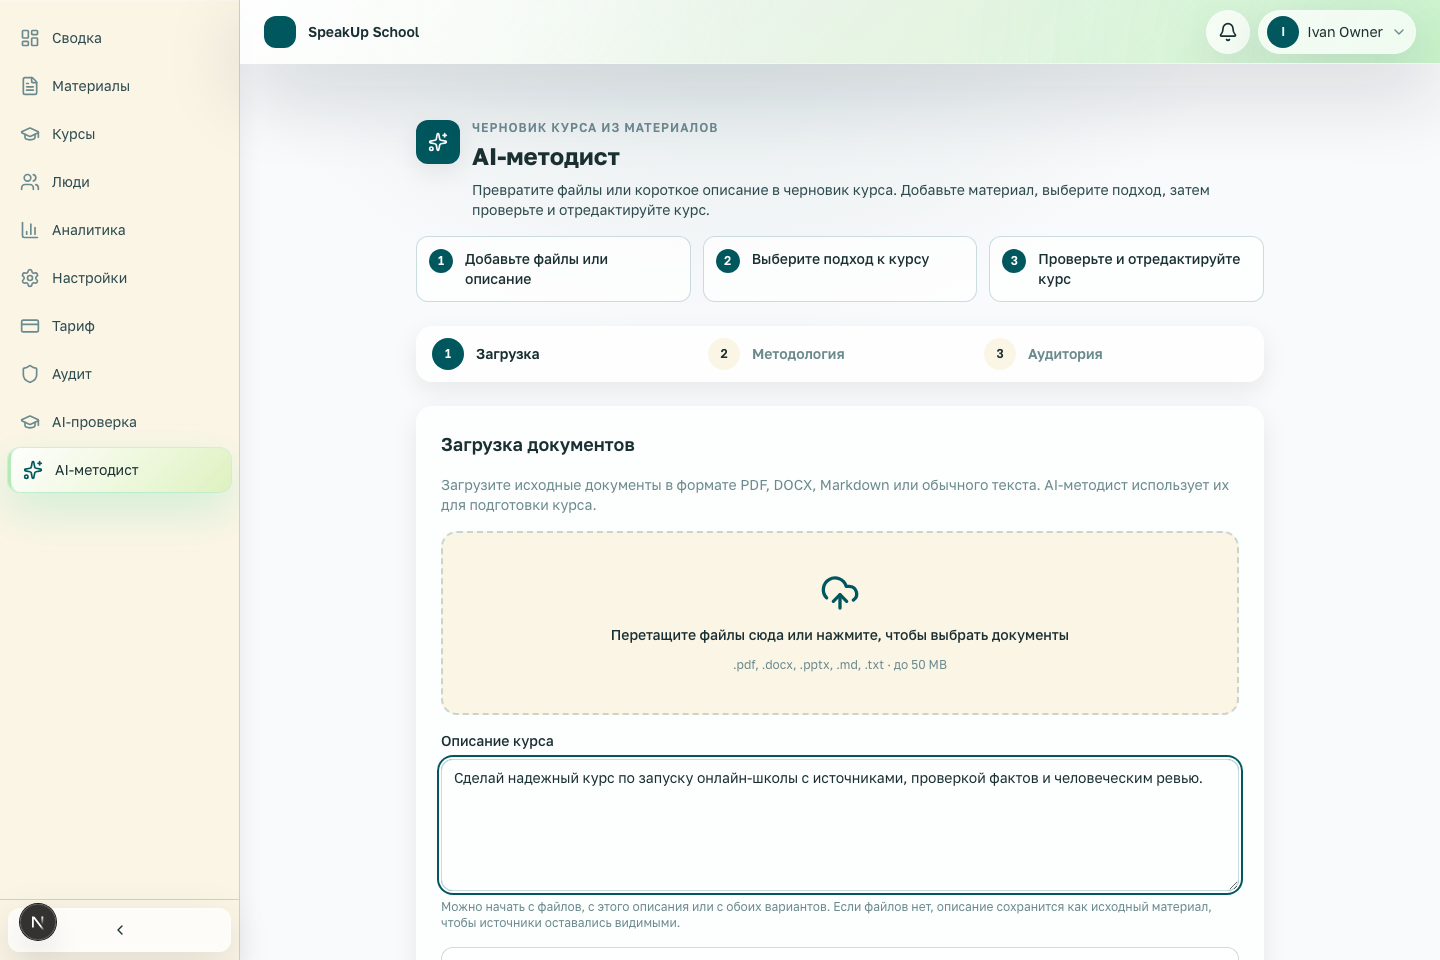
\includegraphics[width=0.98\textwidth]{figures/ui/ai-methodist-01-upload.png}
  \caption{Экран загрузки источников и описания курса для AI-методиста}
  \label{fig:ai-methodist-upload}
\end{figure}

\section*{Л.2 --- Статус пайплайна генерации}

После запуска платформа открывает экран состояния пайплайна
(рисунок~\ref{fig:ai-methodist-status}). На~нём видны этапы анализа
источников, построения структуры, генерации контента, проверки фактов,
ревью и~верификации. В~той~же рабочей области отображаются модель,
токены, оценочная стоимость и~оценка качества.

\begin{figure}[p]
  \centering
  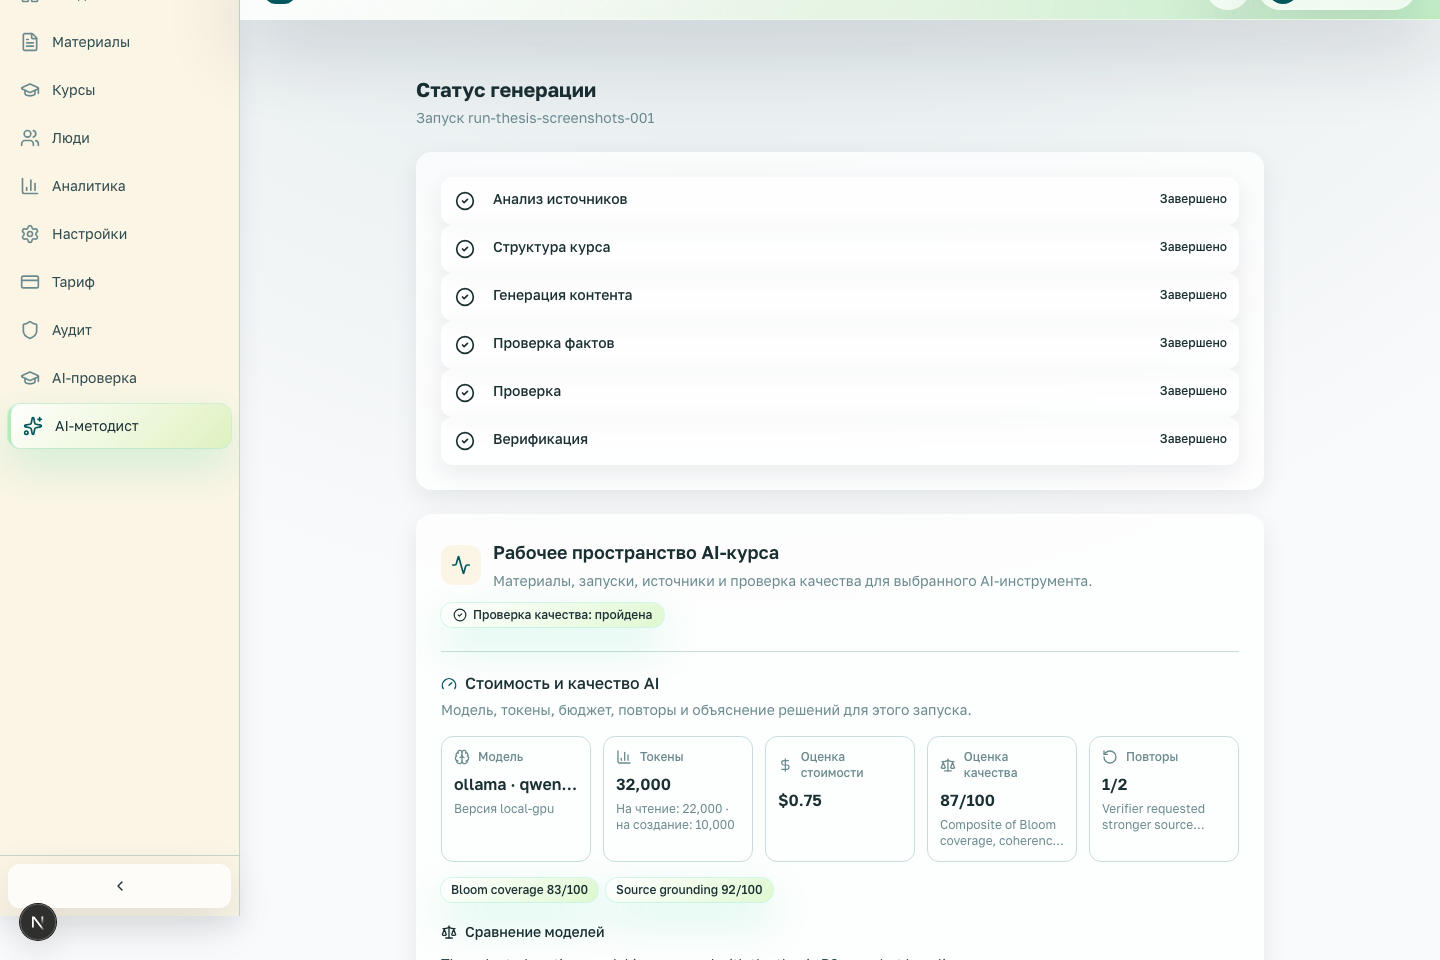
\includegraphics[width=0.98\textwidth]{figures/ui/ai-methodist-02-status.png}
  \caption{Экран статуса генерации, стоимости и качества запуска AI-методиста}
  \label{fig:ai-methodist-status}
\end{figure}

\section*{Л.3 --- Метрики дипломной валидации}

На~рисунке~\ref{fig:ai-methodist-thesis-validation} показан блок
дипломной валидации. Он фиксирует выполнение критериев H1--H3,
включая время до~первого черновика, Bloom coverage, source grounding
и~стоимость относительно ручной разработки. В~том~же интерфейсном
блоке показано paired-сравнение B1/B2/B3/B4 на~одном источнике.

\begin{figure}[p]
  \centering
  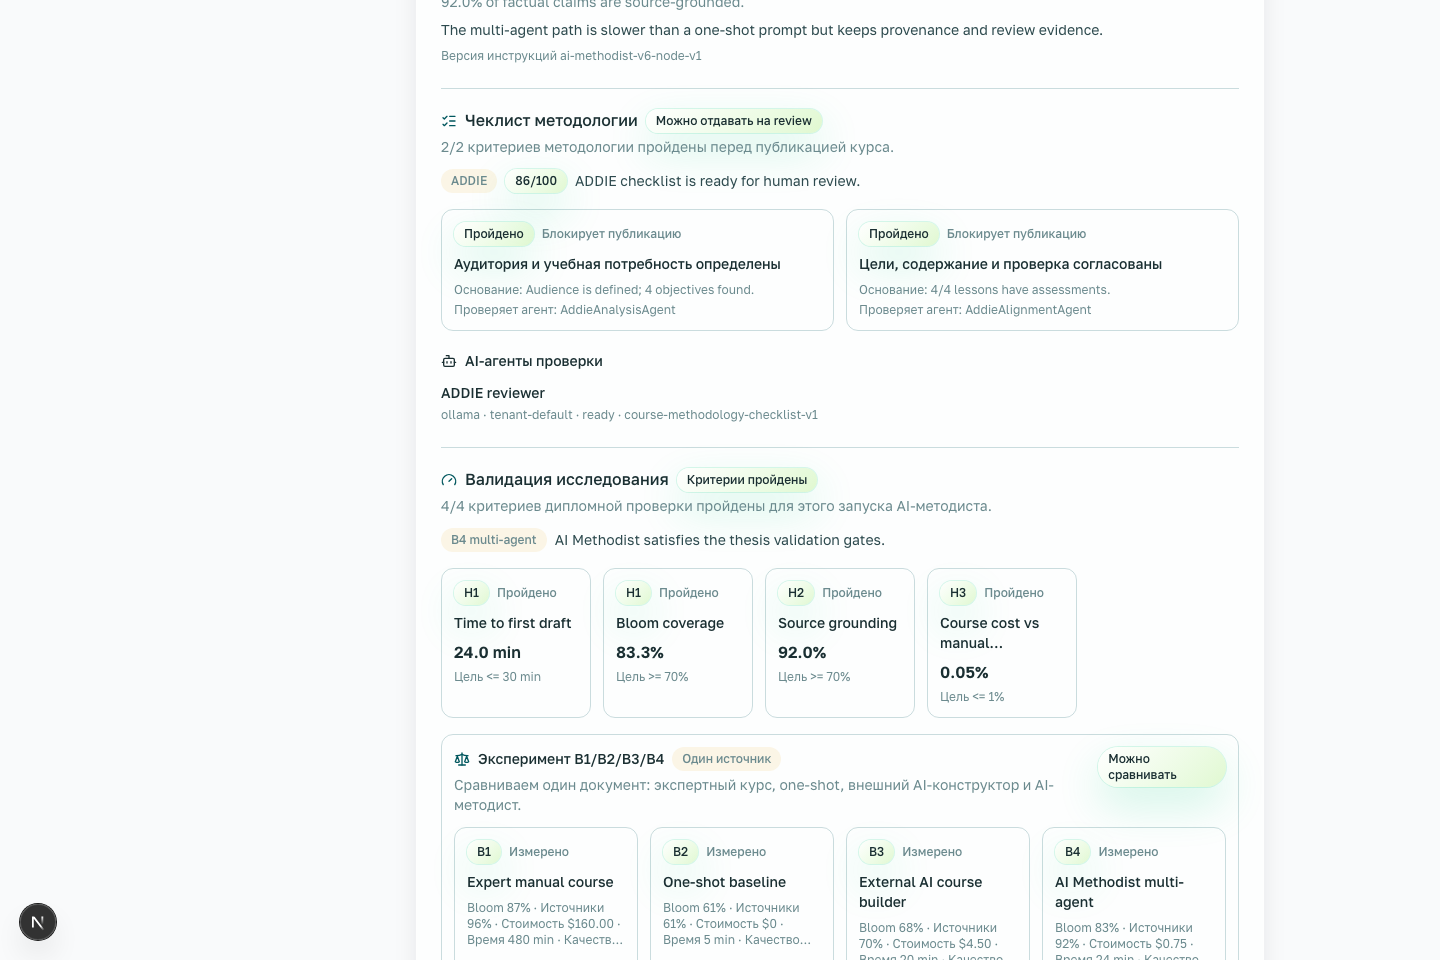
\includegraphics[width=0.98\textwidth]{figures/ui/ai-methodist-03-thesis-validation.png}
  \caption{Метрики дипломной проверки и paired-сравнение B1/B2/B3/B4}
  \label{fig:ai-methodist-thesis-validation}
\end{figure}

\section*{Л.4 --- Quality seal и источники}

На~рисунке~\ref{fig:ai-methodist-quality-seal} показаны загруженный
материал, история запуска, статусы генерации, источники и~итоговый
quality seal перед публикацией. Такой экран нужен комиссии как
подтверждение, что AI-методист не~ограничивается созданием текста:
результат сопровождается проверкой качества и~ссылками на~источники.

\begin{figure}[p]
  \centering
  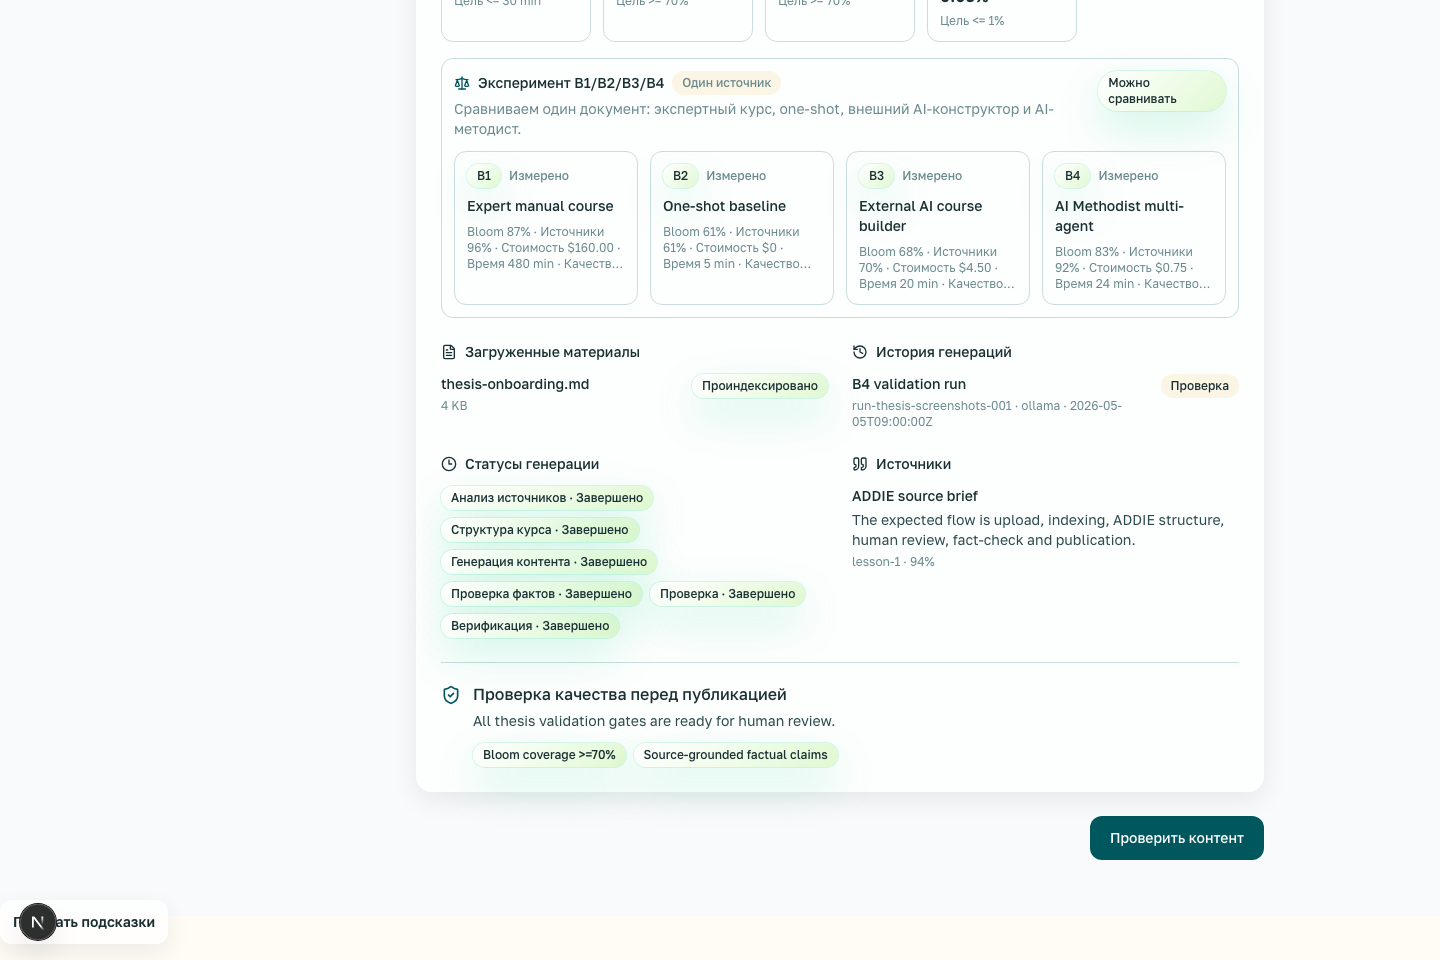
\includegraphics[width=0.98\textwidth]{figures/ui/ai-methodist-04-quality-seal.png}
  \caption{Quality seal, источники и история запуска AI-методиста}
  \label{fig:ai-methodist-quality-seal}
\end{figure}

\section*{Л.5 --- Provenance блоков курса}

На~рисунке~\ref{fig:ai-methodist-block-provenance} показан экран
проверки контента перед публикацией. Для каждого блока курса платформа
отображает источник, страницу, фрагмент, идентификатор запуска и~уровень
уверенности. Если источник отсутствует, интерфейс явно показывает
предупреждение, что блок нельзя считать полностью подтверждённым.

\begin{figure}[p]
  \centering
  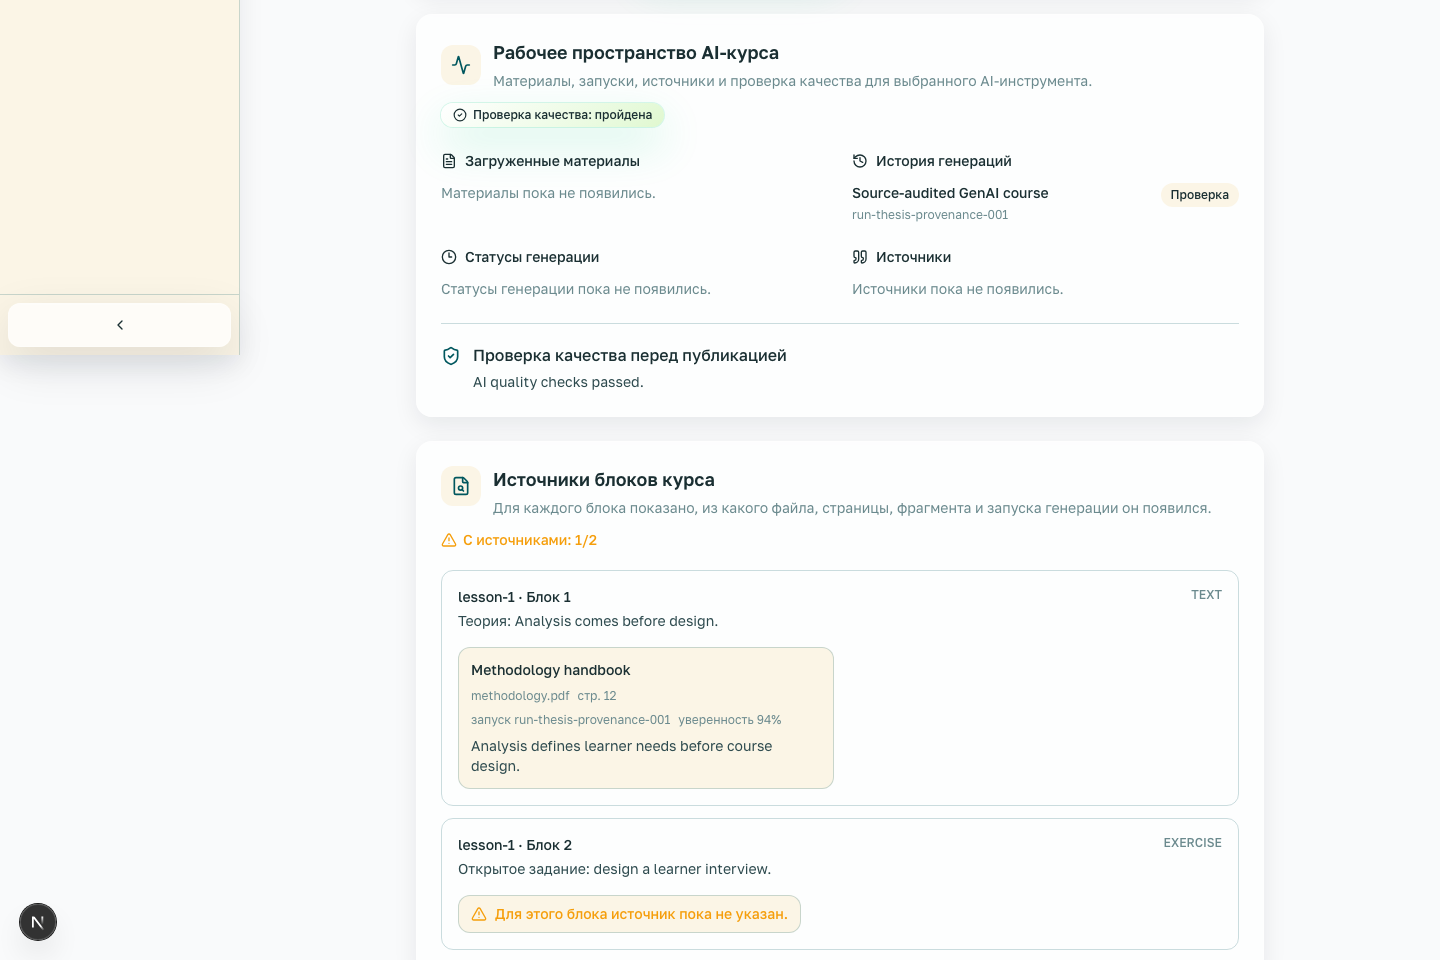
\includegraphics[width=0.98\textwidth]{figures/ui/ai-methodist-06-block-provenance.png}
  \caption{Block-level provenance: источник, страница, фрагмент и предупреждение о неподтверждённом блоке}
  \label{fig:ai-methodist-block-provenance}
\end{figure}
   % Л — Описание экранов MVP и демо-сценарий

\end{document}
